\chapter{Algoritmi di ordinamento}\label{cap:ordinamento}
\section{Il problema dell'ordinamento}

\dfn{Ordinamento}{
	Sia $A$ una sequenza di n numeri $\langle a_{1},a_{2},...,a_{n}\rangle$ con $a_{i}\in \mathbb{Z} \quad \forall \; 1 \leq i \leq n$. \textbf{Ordinare} $A$ significa trovare una sequenza $A'$ chiamata \textbf{permutazione ordinata} di $A$, ovvero un riarrangiamento $\langle a'_{1}, a'_{2},...,a'_{n}\rangle$ tale che
	\begin{equation}\label{condizioneordinamento}
		a'_{1}\leq a'_{2} \leq \cdots \leq a'_{n}
	\end{equation}
}

Per ordinare una sequenza si può pensare di generare tutte le permutazioni possibili a partire da tale sequenza e verificare la proprietà di ordinamento \ref{condizioneordinamento}. Da questa idea possiamo dire con certezza che almeno un algoritmo che risolva il problema dell'ordinamento esista dato che, essendo l'ordinamento totale esisterà sicuramente una soluzione. Ovviamente questo approccio è tanto banale quanto complesso. Algoritmi di questo tipo vengono chiamati \textbf{algoritmi di forza bruta (brute force)}.

Nel caso del problema della massima sottosequenza contigua visto in \ref{sottosequenzecontigue}, l'algoritmo di forza bruta aveva un costo quadratico. In questo caso invece, la differenza è abissale. Data una sequenza di $n$ elementi il numero di permutazioni sarà $n!$, controllare la condizione \ref{condizioneordinamento} implica scorrere ogni elemento di ciascuna permutazione raggiungendo così il costo di $\Omega(n \cdot n!)$ che è molto ma molto grande rispetto ad $n^{2}$.

Nel corso di questo capitolo si vedrà che esistono algoritmi più ``sensati'' per la ricerca di una sequenza ordinata. Il problema da porsi sarà quello della loro \textit{costruzione}. Tutti gli algoritmi che si vedranno in questo capitolo avranno un tempo limitato superiormente da $n^{2}$, quindi sarà: $T(n)=O(n^{2})$.  L'idea alla base sarà quella di ordinare mediante l'utilizzo del \emph{confronto}, volta per volta, di coppie di elementi. Chiaramente, nel migliore dei casi il costo sarà lineare (meno di così non sarà possibile scendere). Questa analisi ci permette quindi di limitare l'intervallo all'interno del quale selezionare algoritmi  che siano ``sensati''.

\section{Insertion Sort}
L'algoritmo \textbf{Insertion sort} è un buon metodo per ordinare un piccolo numero di elementi. La sua idea basilare è molto banale ed è simile al modo in cui molte persone ordinano le carte: preso un mazzo di carte, si inseriscono le carte nella loro posizione corretta una dopo l'altra dopo averle confrontate con quelle precedentemente ordinate. In ogni momento quindi, l'algoritmo vede la sequenza divisa in due parti: una ordinata e una disordinata. Consideriamo quindi una sequenza $A$, l'algoritmo \textsc{Insertion Sort} (Algoritmo \ref{alg:insertsort}) ordina i numeri di input \textbf{in place}, nel  senso che i numeri sono risistemati all'interno dell'array $A$ senza l'utilizzo di alcuna struttura ausiliaria. Quando la procedura è completata, l'array di input $A$ contiene la sequenza di output ordinata.

\begin{lstlisting}[caption={\textsc{InsertionSort}(A,n)},language=asd,label=alg:insertsort]
for j=2 to n do
	elem = A[j]
	// Inserisce A[j] nella sequenza ordinata A[1,...,j-1]
	i = j-1
	while i @$\geq$@ 1 && elem < A[i] do
		A[i+1] = A[i]
		i = i-1
	A[i+1] = elem
\end{lstlisting}

\begin{center}
	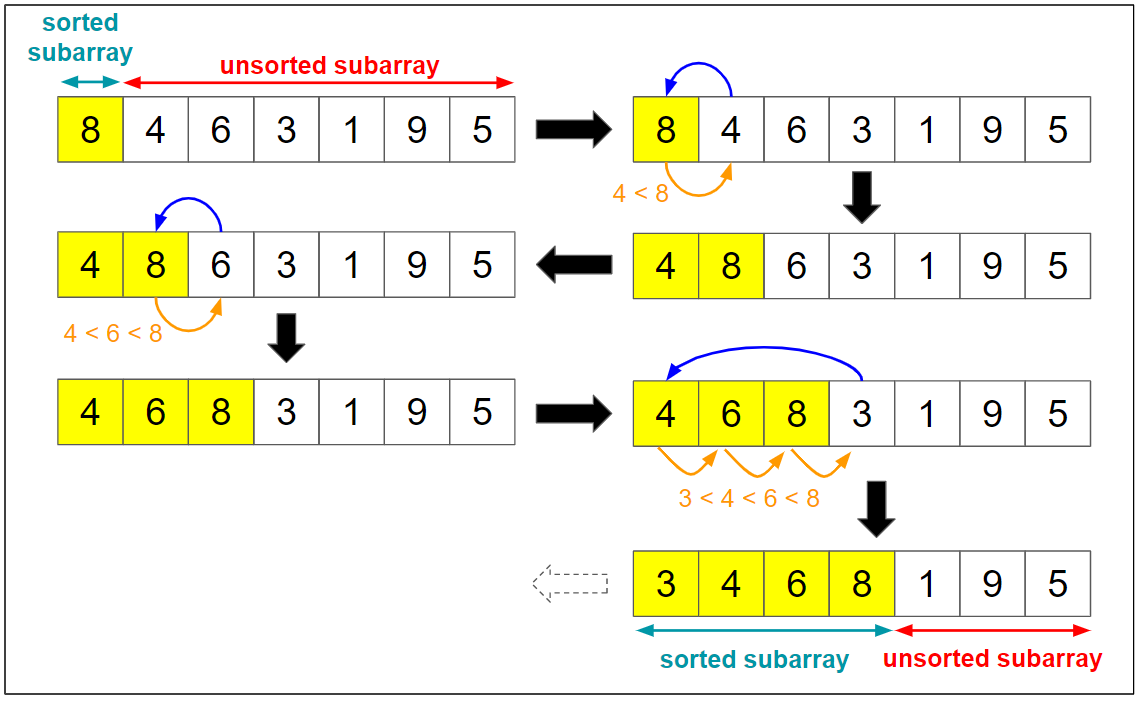
\includegraphics[scale=.3]{res/InsertionSort1}
	\captionof{figure}{Esempio di applicazione di \textsc{Insertion Sort}}
\end{center}

\subsection{Invarianti di ciclo e correttezza di \textsc{InsertionSort}}
Il tempo richiesto dalla procedura \textsc{Insertion-Sort} dipende dall'input: occorre più tempo per ordinare un migliaio di numeri che tre numeri. Inoltre, \textsc{Insertion-Sort} può richiedere quantità di tempo differenti per ordinare due sequenze di input della stessa dimensione a seconda della \textit{qualità} della sequenza. Infatti non si può dire a priori il numero di esecuzioni del ciclo \texttt{while} al rigo 5 dell'Algoritmo \ref{alg:insertsort}.

In casi come questi si andranno a fare due analisi distinte e separate, una prima per quelle classi di istanze ``buone'' che offriranno tempi di esecuzioni brevi e una seconda analisi per quelle istanze dette anche ``peggiori''. Bisogna capire però come \textit{formalizzare la dipendenza dalla bontà dell'input del tempo}. Per rispondere a questa domanda si introducono una serie di parametri, detti $t_{j}$, che indicano il numero di iterazioni della testa del ciclo \texttt{while}, \textit{fissato} l'indice $j$.

Poiché abbiamo che $j$ varia da $2$ a $n$ avremo rispettivamente: $t_{2},...,t_{n}$. Complessivamente la testa del \texttt{while} sarà eseguita quindi $\sum_{j=2}^{n}t_{j}$ volte. Una volta introdotti questi parametri possiamo dire quindi che le istruzioni 6 e 7 saranno eseguite rispettivamente $\sum_{j=2}^{n}(t_{j}-1)$ volte. Si ha così un \textbf{prospetto parametrico} del costo istruzione per istruzione.

\begin{center}
	\begin{tblr}{hlines,vlines,cells={mode=math},row{1}={primary!80!white},column{1}={primary!80!white}}
	\textbf{Istruzione} & \textbf{\# Operazioni} & \textbf{Esecuzioni} \\
	1 & 2 & n \\
	2 & 2 & n-1 \\
	3 & 2 & n-1 \\
	5 & 4 & \sum_{j=2}^{n} t_{j}\\
	6 & 3 & \sum_{j=2}^{n} t_{j-1}\\
	7 & 1 & \sum_{j=2}^{n} t_{j-1}\\
	8 & 2 & n-1\\
\end{tblr}
\end{center}

Il tempo di esecuzione dell'algoritmo è la somma dei tempi di esecuzione per ogni istruzione eseguita.

Per calcolare $T(n)$ sommiamo i prodotti delle colonne \textbf{Numero operazioni} e \textbf{Numero di volte}:
\begin{eqnarray}\label{eq:FormaGenericaInsertSort}
	T(n) &=& 2n+2(n-1)+2(n-1)+4\sum_{j=2}^{n}t_{j}+3\sum_{j=2}^{n}(t_{j}-1)+\sum_{j=2}^{n}(t_{j}-1)\nonumber \\
	&=& 9n-7+4\sum_{j=2}^{n}t_{j}+4\sum_{j=2}^{n}(t_{j}-1)
\end{eqnarray}
L'equazione \ref{eq:FormaGenericaInsertSort} non è una espressione precisa poiché dipendente dai parametri $t_{j}$ però a partire da questa formula possiamo iniziare a fare le due analisi distinte, una per il \textbf{caso peggiore} e una per il \textbf{caso migliore}.
\subsubsection{Caso peggiore}
Nel caso peggiore, ovvero quello di una sequenza ordinata in senso inverso, nella testa del \texttt{while} la condizione $elem<A[i]$ è sempre vera, quindi la condizione farà sempre entrare nel \texttt{while} e il ciclo dipenderà unicamente dall'indice $i\geq 1$. L'algoritmo dovrà confrontare ogni elemento $A[j]$ con ogni elemento dell'intera sottosequenza ordinata $A[1..j-1]$ e quindi sarà $t_{j}=j$ per $j=2,3,...,n$.

Sarà quindi:
\begin{eqnarray}
	T(n) &=& 9n-7+4\sum_{j=2}^{n}j+4\sum_{j=2}^{n}(j-1) \nonumber \\
	&=& 9n -7 + 4\cdot \bigl( \frac{n(n+1)}{2} -1\bigl) +4 \cdot \frac{n(n-1)}{2} \nonumber \\
	&=& 9n -7 + 4 \cdot ((n^{2}+n)-2)+4 \cdot \frac{n(n-1)}{2} \nonumber \\
	&=& 9n - 7 + 4n^{2}+ 4n -8 +2n^{2}-2n \nonumber \\
	&=& 6n^{2}+11n-15
\end{eqnarray}
Possiamo concludere quindi che, nel caso peggiore $T(n)=O(n^{2})$.

\subsubsection{Caso migliore}
In \textsc{Insertion-Sort} il caso migliore si verifica se l'array è già ordinato. Per ogni $j=2,3,...,n$, troviamo che $A[i]<elem$ nella testa del ciclo \texttt{while}, quando $i$ ha il suo valore iniziale $j-1$. Quindi $t_{j}=1$ per $j=2,...,n$ e il tempo di esecuzione nel caso migliore è:
\begin{eqnarray}
	T(n) &=& 9n-7+4\sum_{j=2}^{n}t_{j}+4\sum_{j=2}^{n}(t_{j}-1) \nonumber \\
	&=& 9n-7+4 \sum_{j=2}^{n}1+4\sum_{j=2}^{n}(0) \nonumber \\
	&=& 9n-7+n-1 \nonumber \\
	&=& 10n -8
\end{eqnarray}
Nel caso migliore quindi $T(n)=O(n)$.

\subsubsection{Caso medio}
L'equazione \ref{eq:FormaGenericaInsertSort} ci aveva dato una formula generale, dipendente dai parametri $t{j}$, del costo di \textsc{Insertion-Sort}. Ci si può chiedere però se, fissato l'indice $j$, possa esistere un parametro $t_{medio}$. Nulla vieta di calcolare $t_{medio}$ come la media aritmetica dei vari parametri, assumendo una equiprobabilità delle tipologie di input:
\begin{displaymath}
	t_{medio}=\frac{\sum_{k=1}^{j}k}{j}=\frac{\frac{j(j+1)}{2}}{j}=\Bigl \lfloor \frac{j+1}{2}\Bigl \rfloor
\end{displaymath}
E così la \ref{eq:FormaGenericaInsertSort} diventa:
\begin{eqnarray}
	T_{medio}(n)&=& 9n-7+4\sum_{j=2}^{n}\frac{j+1}{2}+4\sum_{j=2}^{n}\bigl(\frac{j+1}{2}-1\bigl)\nonumber \\
	&=& 9n-7+2\sum_{j=2}^{n}(j+1)+2\sum_{j=2}^{n}(j-1)\nonumber \\
	&=& 9n-7+2\sum_{j=2}^{n}(j+1)+2\sum_{j=1}^{n-1}j \nonumber\\
	&=& 9n-7+2\sum_{j=2}^{n}(j+1)+\frac{n(n-1)}{2}
\end{eqnarray}
Possiamo dire quindi che anche nel caso medio \textsc{Insertion-Sort} ha un comportamento quadratico: $T_{medio}(n)=O(n^{2})$.

\section{Merge Sort}
Per \textsc{Insertion Sort} abbiamo usato un approccio \textbf{incrementale}: dopo avere ordinato il sottoarray $A[1..j-1]$, abbiamo inserito un singolo elemento $A[j]$ nella posizione appropriata, ottenendo il sottoarray ordinato $A[1,...,j]$. L'algoritmo \textsc{Merge-Sort} è un tipo di algoritmo come quelli visti nel Capitolo \ref{cap:ricorrenze}, ovvero un algoritmo ricorsivo. La ricorsione, in questo caso, ridurrà di molto il tempo di esecuzione rispetto ad \textsc{Insertion-Sort} nel caso peggiore.


L'algoritmo \textsc{MergeSort} è conforme al paradigma divide et impera. Esso opera nel modo seguente:
\begin{itemize}
	\item \textbf{Divide:} divide la sequenza degli $n$ elementi da ordinare in due sottosequenze di $n/2$ elementi ciascuna.
	\item \textbf{Impera:} ordina le due sottosequenze in modo ricorsivo utilizzando l'algoritmo merge sort.
	\item \textbf{Combina:} fonde le due sottosequenze ordinate per generare la sequenza ordinata.
\end{itemize}

La ricorsione tocca il fondo quando la sequenza da ordinare ha lunghezza 1, in quel caso non c'è nulla da fare, in quanto ogni sequenza di lunghezza 1 è già ordinata.
\begin{lstlisting}[caption={\textsc{MergeSort}(A,p,r)},language=asd,label=alg:mergesort]
	// Verifica dell'intervallo
	if p<r then
		q = @$\lfloor$@ p+r / 2 @$\rfloor$@
		MergeSort(A,p,q)
		MergeSort(A,q+1,r)
		Merge(A,p,q,r)
\end{lstlisting}


L'operazione chiave dell'algoritmo \textsc{Merge Sort} è la \textit{fusione} di due sottosequenze ordinate nel passo ``combina''. Per effettuare la fusione, utilizziamo una procedura ausiliaria chiamata \textsc{Merge}$(A,p,q,r)$, dove $A$ è un array e $p$, $q$, $r$ sono indici dell'array tali che $p \leq q \leq r$. La procedura assume che i sottoarray $A[p..q]$ e $A[q+1...r]$ siano ordinati; li \textbf{fonde} per formare un unico array ordinato che sostituisce il sottoarray corrente $A[p..r]$.

\subsection{Correttezza dell'algoritmo}
Poiché $p$ ed $r$ indicano l'indice iniziale e finale della sequenza $A$ possiamo dire che $A$ ha $r-p+1$ elementi. Affinché \textsc{Merge-Sort} funzioni bisogna garantire la convergenza del passo ``divide'', ovvero:
\begin{displaymath}
	r-p+1>\underbrace{q-p+1}_{1^{a} sottosequenza} \wedge \underbrace{r-p+1}_{2^{a} sottosequenza} > \underbrace{r-q}_{r-(q+1)+1}
\end{displaymath}

dove $$q=\bigl \lfloor \frac{p+r}{2}\bigl \rfloor$$
e sappiamo che $$\bigl \lfloor\frac{p+r}{2}\bigl \rfloor \leq \frac{p+r}{2}$$
ma allora risulta:
\begin{displaymath}
	r-p+1 > \frac{p+r}{2}-p+1 \implies 2r>p+r \implies r>p
\end{displaymath}
ed essendo la nostra ipotesi proprio $p<r$ abbiamo dimostrato la prima implicazione. Analogamente si procede per la seconda:
\begin{displaymath}
	r-p+1>r-\frac{p+r}{2} \implies -p > -\bigl ( \frac{p+r}{2}+1 \bigl) \implies 2p<p+r+2 \implies p<r+2
\end{displaymath}

Resta solo da dimostrare che, per qualsiasi input, l'algoritmo faccia un numero finito di chiamate ricorsive e che quindi, prima o poi, raggiungerà il caso base. Quando r è molto vicino a p, ovvero quando $r<p+1$ è evidente che sarà $q=\lfloor (p+r)/2 \rfloor = p$ e quindi entrambe le chiamate ricorsive non verranno effettuate poiché la condizione del blocco condizionale if sarà alla prima chiamata $p<p$ ed alla seconda $p+1<r$ (entrambe ovviamente false).

\subsection{L'algoritmo \textsc{Merge}}
\begin{lstlisting}[caption={\textsc{Merge}(A,p,q,r)},language=asd]
	i=p
	k=p
	j=q+1
	while i <= q && j <= r do
		if A[i] <= A[j] then
			B[k] = A[i]
			i=i+1
		else
			B[k] = A[j]
			j=j+1
		k =k+1
	if i < q then
		j=i
	while k <= r do
		B[k] = A[j]
		j = j+1
		k = k+1
\end{lstlisting}

Il costo di esecuzione di \textsc{Merge} è ovviamente lineare poiché si andranno a fare almeno $n$ scritture in memoria:
\begin{displaymath}
	T_{Merge}=\Theta(n)
\end{displaymath}

\subsection{Analisi del costo di \textsc{Merge Sort}}
Per calcolare il tempo di esecuzione dell'algortimo \textsc{Merge Sort} (Algoritmo \ref{alg:mergesort}) si definisce una funzione di ricorrenza del tipo:
\begin{displaymath}
	T_{MergeSort}(N)=
	\begin{cases}
		\Theta(1) & \mbox{ se } n \leq 1\\
		T_{Merge}(N)+\Theta(1) +2 T_{MergeSort}(N/2) & \mbox{ se } n > 1
	\end{cases}
\end{displaymath}
che, sommando $T_{Merge}(N)+\Theta(1)$, diventa:
\begin{equation}\label{eqric:mergesort}
	T_{MergeSort}(N)=
	\begin{cases}
		\Theta(1) & \mbox{ se } n \leq 1\\
		2 T_{MergeSort}(N/2) + \Theta(N) & \mbox{ se } n > 1
	\end{cases}
\end{equation}
Notiamo che l'equazione \ref{eqric:mergesort} è uguale all'equazione \ref{eqricorrenza1} vista nel Capitolo \ref{cap:ricorrenze}. Possiamo concludere quindi che il costo di esecuzione di \textsc{Merge Sort} è:
\begin{displaymath}
	T_{MergeSort}=\Theta(n \log_{2}N)
\end{displaymath}

\section{Selection Sort}
L'idea che sta alla base dell'algoritmo \textsc{Selection Sort} può essere visto come il duale di quella dell'algoritmo \textsc{Insertion Sort}. Infatti, selezionata una posizione della sequenza si trova successivamente l'elemento da metterci dentro.

Come si vede in Figura \ref{fig:SelectionSort}, se iniziamo dall'ultima posizione, ovvero $N$, allora si dovrà trovare il massimo elemento della sequenza evidenziata in azzurro e poi scambiarlo con quello in posizione $N$ (se avessimo preso l'elemento in prima posizione allora si sarebbe dovuto cercare l'elemento più piccolo). Il procedimento si ripete riducendo di volta in volta la sequenza da ordinare che avrà dimensione $N$ poi $N-1$ fino a quando, arrivati alla posizione $2$, non si sarà ottenuta la sequenza ordinata (infatti alla fine dell'ultima iterazione il minimo già si troverà nella posizione $1$).

\begin{figure}[ht!]
	\centering
	\subfloat[All'inizio l'array non è ordinato, selezioniamo quindi l'ultima cella dove dovrebbe trovarsi il massimo.]
	{
		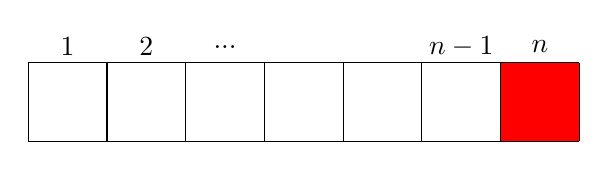
\begin{tikzpicture}
			%\fill[blue, nearly transparent] (0,0) rectangle (6,-1);
			\fill[red] (6,0) rectangle (7,-1);
			\draw (0,0) grid (7,-1);
			\node at (0.5,0.2) {1};
			\node at (1.5,0.2) {2};
			\node at (2.5,0.2) {...};
			\node at (5.5,0.2) {$n-1$};
			\node at (6.5,0.2) {$n$};
		\end{tikzpicture}
	} \hfil
	\subfloat[Chiamo l'algoritmo \textsc{FindMax} sulla sequenza $1,n-1$: se il massimo si trova nella cella 0, evidenziata in verde, eseguo lo swap con la cella rossa.]
	{
		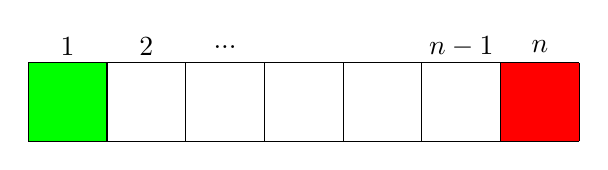
\begin{tikzpicture}
			\fill[green] (0,0) rectangle (1,-1);
			%\fill[blue, nearly transparent] (1,0) rectangle (6,-1);
			\fill[red] (6,0) rectangle (7,-1);
			\draw (0,0) grid (7,-1);
			\node at (0.5,0.2) {1};
			\node at (1.5,0.2) {2};
			\node at (2.5,0.2) {...};
			\node at (5.5,0.2) {$n-1$};
			\node at (6.5,0.2) {$n$};
		\end{tikzpicture}
		}\\
		\subfloat[A questo punto il massimo si trova in posizione corretta.]
		{
			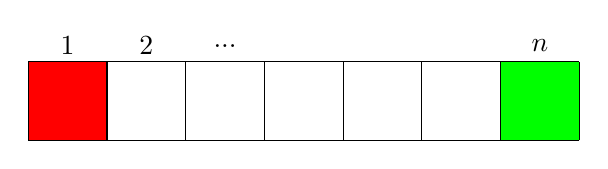
\begin{tikzpicture}
				\fill[red] (0,0) rectangle (1,-1);
				%\fill[blue, nearly transparent] (1,0) rectangle (6,-1);
				\fill[green] (6,0) rectangle (7,-1);
				\draw (0,0) grid (7,-1);
				\node at (0.5,0.2) {1};
				\node at (1.5,0.2) {2};
				\node at (2.5,0.2) {...};
				\node at (6.5,0.2) {$n$};
			\end{tikzpicture}
		} \hfil
	\subfloat[Riduciamo la sottosequenza e ripetiamo il ragionamento. La parte evidenziata in verde risulta già ordinata mentre resta da ordinare la parte evidenziata in giallo.]
	{
		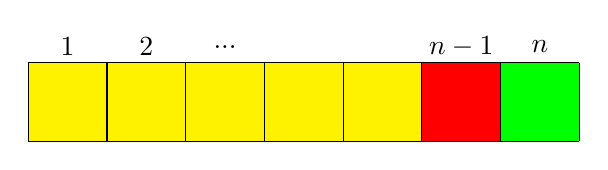
\begin{tikzpicture}
			\fill[red] (5,0) rectangle (6,-1);
			\fill[yellow] (0,0) rectangle (5,-1);
			\fill[green] (6,0) rectangle (7,-1);
			\draw (0,0) grid (7,-1);
			\node at (0.5,0.2) {1};
			\node at (1.5,0.2) {2};
			\node at (2.5,0.2) {...};
			\node at (5.5,0.2) {$n-1$};
			\node at (6.5,0.2) {$n$};
		\end{tikzpicture}
	}
	\caption{Esempio di applicazione dell'Algoritmo \ref{alg:selectionsort}}\label{fig:SelectionSort}
\end{figure}

\begin{minipage}{.4\textwidth}
	\begin{lstlisting}[caption={\textsc{SelectionSort}(A,n)},language=asd,label=alg:selectionsort]
		for i =n to 2 do
			j = FindMax(A,i)
			Swap(A,i,j)
	\end{lstlisting}
\end{minipage}
\begin{minipage}{.4\textwidth}
	\begin{lstlisting}[caption={\textsc{FindMax}(A,n)},language=asd,label=alg:findmax]
		max = i
		for i = 2 to n
		if A[max] < A[i] then
			max = i
		return max
	\end{lstlisting}
\end{minipage}

\subsection{Analisi del costo di \textsc{SelectionSort}}
Poiché sappiamo che la scelta del massimo non può essere fatta con un algoritmo meno che lineare (poiché bisogna confrontare comunque ogni elemento della successione) sembrerebbe che questa sia una soluzione ottimale. Questo algoritmo però è un esempio di come usare usare soluzioni ottime per dei sottoproblemi non rende l'algoritmo ottimale. Ma ciò non significa che l'idea alla base sia pessima; infatti nella sezione \ref{sez:HeapSort} vedremo come abbassare il tempo di esecuzione ad un $\Theta(n \log_{2}n)$.

Si ha quindi:
\begin{eqnarray}
	T_{SS}(N) &=& \Theta(N)+\sum_{i=2}^{N} T_{FindMax}(i)+ \Theta(1) \nonumber \\
	&=& \Theta(N)+ \Theta \Bigl(\sum_{i=2}^{N} i \Bigr) \nonumber \\
	&=& \Theta(N) + \Theta \Biggl( \Bigl(\sum_{i=1}^{N}i \Bigr) -1 \Biggr) \nonumber \\
	&=& \Theta(N) + \Theta \bigl(\frac{n(n+1)}{2} -1\bigr) \nonumber \\
	&=& \Theta(n^{2})
\end{eqnarray}

\section{Heap Sort}\label{sez:HeapSort}
L'algoritmo \textsc{SelectionSort} (Algoritmo \ref{alg:selectionsort}) si è dimostrato essere il peggior algoritmo visto fino a questo momento. Il suo problema non è legato all'idea che sta alla sua base quando piuttosto alla sua \textit{implementazione}. Il punto è che l'algoritmo \textsc{FindMax} (Algoritmo \ref{alg:findmax}) \textbf{non conserva informazioni sull'ordinamento parziale}. L'algoritmo \textsc{HeapSort} cerca di risolvere questa problematica introducendo una struttura dati detta \textbf{heap} (mucchio), per gestire la conservazione di queste informazioni e \textit{ridurre il numero di confronti per la ricerca del massimo}.

\subsection{Gli alberi heap}
Dalle proprietà degli alberi binari pieni\footnote{Vedi \ref{alberi_binari_prop}} si ha che:
\begin{eqnarray}
	N_{\mbox{{\footnotesize nodi interni}}}&=& \sum_{i=0}^{h-1} 2^{i}= 2^{h}-1\\
	h&=&\lfloor \log_{2}n\rfloor \label{altezzaheap} \\
	N_{\mbox{{\footnotesize nodi}}}&=& 2^{h+1}-1 \label{eq:noditree}
\end{eqnarray}
da cui si evince che non tutti gli insiemi possono essere rappresentati da un albero binario pieno (ad esempio un insieme con 5 elementi).

Per garantire che insiemi di ogni cardinalità possano essere rappresentati da un albero heap si usano gli \textbf{alberi binari completi}, ovvero un albero sul quale si impone un rilassamento dei vincoli degli alberi binari pieni. In particolare:
\begin{itemize}
	\item Tutte le foglie sono a livello $h$ oppure $h-1$;
	\item Tutti i nodi interni hanno grado 2 tranne al più un nodo.
\end{itemize}

\dfn{Albero heap}{
	Un \textbf{albero heap} è un albero binario di altezza $h$ tale che, per ogni nodo $i$:
	\begin{enumerate}
		\item tutte le foglie hanno profondità $h$ o $h-1$;
		\item tutti i nodi interni hanno grado $2$, eccetto al più uno;
		\item entrambi i nodi $j$ e $k$ figli di $i$ sono \emph{non maggiori} di $i$.
	\end{enumerate}
}


\begin{osservation}
	Le prime due condizioni definiscono la forma dell'albero, in particolare un albero completo  mentre la terza condizione definisce l'\textbf{architettura} dell'albero. In definitiva, un albero heap è un albero binario completo tale che per ogni nodo entrambi i figli non sono maggiori del padre (proprietà di ordinamento parziale). 
\end{osservation}

\begin{center}
	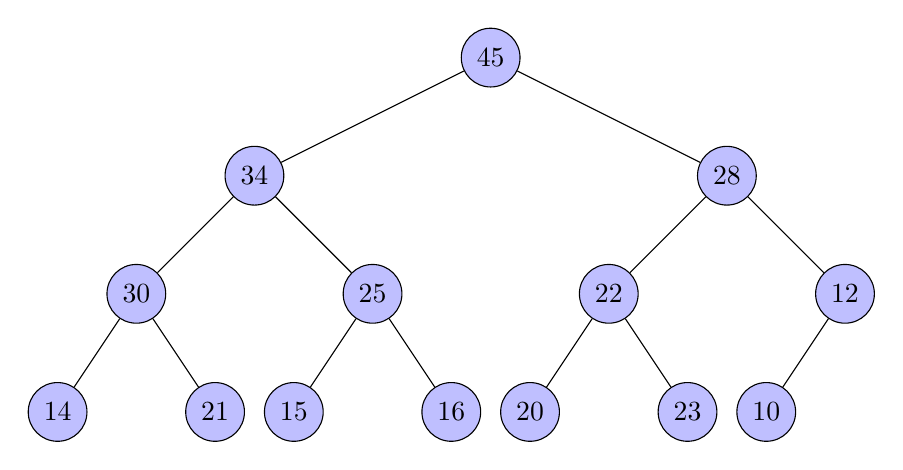
\begin{tikzpicture}
		[every node/.style={circle,draw,fill=blue!25!white,minimum size=0.5cm},
		level/.style={sibling distance=60mm/#1}]
		\node{45}
		child{
			node{34}
			child{
				node{30}
				child{node{14}}
				child{node{21}}
			}
			child{
				node{25}
				child{node{15}}
				child{node{16}}
			}
		}
		child{
			node{28}
			child{
				node{22}
				child{node{20}}
				child{node{23}}
			}
			child{
				node{12}
				child{node{10}}
				child[missing]
			}
		};
	\end{tikzpicture}
	\captionof{figure}{Esempio di albero heap}\label{fig:heap}
\end{center}

\subsection{Il problema della rappresentabilità}
Dato un qualsiasi $n \in \mathbb{N}$, siamo sicuri che tutti gli insiemi possono essere rappresentati da un albero binario completo? In generale infatti possiamo saltare da alberi pieni contenenti $2^{h+1}-1$ nodi ad alberi con $2^{(h+1)+1}-1=2^{h+2}-1$ nodi. Non esiste però nessun albero pieno con un numero di nodi compreso tra $2^{h+1}-1$ e $2^{h+2}-1$. Se si riuscisse a dimostrare che si possono costruire alberi binari completi a partire da $2^{h+1}-1$ nodi allora si potrebbe garantire la proprietà ricercata.

Sia $h=1$ Allora è possibile considerare due alberi pieni contenenti:
\begin{displaymath}
	2^{h+1}-1 = 2^{1+1}-1=2^{2}-1=4-1=3
\end{displaymath}
e
\begin{displaymath}
	2^{h+2}-1 = 2^{1+2}-1=2^{3}-1=8-1=7
\end{displaymath}
nodi ciascuno come mostrato in figura:

\begin{center}
\begin{minipage}{.45\textwidth}
	\centering
	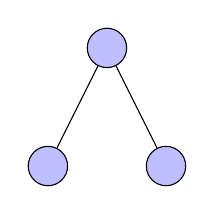
\begin{tikzpicture}
	[every node/.style={circle,draw,fill=blue!25!white,minimum size=0.5cm}]
	\node{}
	child{
		node{}
	}
	child{
		node{}	
	};
\end{tikzpicture}
\end{minipage}
\hfil
\begin{minipage}{.45\textwidth}
	\centering
	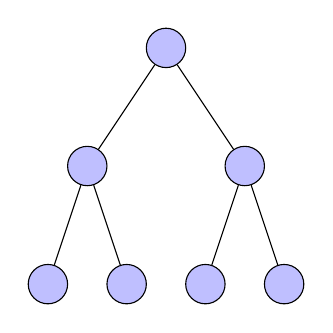
\begin{tikzpicture}
		[every node/.style={circle,draw,fill=blue!25!white,minimum size=0.5cm},
		level/.style={sibling distance=20mm/#1}]
		\node{}
		child{
			node{}
			child{
				node{}
			}
			child{
				node{}	
			}
		}
		child{
			node{}
			child{
				node{}
			}
			child{
				node{}
			}
		};
	\end{tikzpicture}
\end{minipage}
\end{center}

Ad esempio, aggiungendo un nodo all'albero pieno con tre nodi si ottiene un albero completo avente 4 nodi compreso tra i due alberi pieni. Procedendo induttivamente con questa estensione possiamo dire quindi che il problema della cardinalità è stato risolto: dall'arbitrarietà di $h$ possiamo costruire alberi completi per ogni numero di nodi $x$ tali che:
\begin{displaymath}
	2^{h+1}-1 \leq x \leq 2^{h+2}-1
\end{displaymath}

Il rilassamento che abbiamo fatto garantisce la proprietà \ref{altezzaheap}? Bisogna dimostrare cioè che anche per un albero completo vale la proprietà di essere \textit{il più corto con quel numero di nodi} e che quindi è possibile ancora scrivere l'altezza in corrispondenza del numero di nodi. Chiaramente, negli alberi completi non vale più la proprietà  \ref{eq:noditree} poiché abbiamo dimostrato che un albero completo \textbf{può avere un numero di nodi qualsiasi}. Ma è vero anche che $2^{h}\leq n \leq 2^{h+1}$ e quindi $n$ o è una potenza di due o si trova tra due potenze di due.

Dunque, sapendo che $\forall n \in \mathbb{N}, \exists h \geq 0$
\begin{displaymath}
	2^{h}-1 \leq n \leq 2^{h+1}-1 \Rightarrow 2^{h+1}-1 \leq n \leq 2^{h+2}-1
\end{displaymath}
applicando il logaritmo a tutti i membri:
\begin{displaymath}
	\log(2^{h+1}-1) \leq \log n \leq \log(2^{h+1}-1) \Rightarrow \lfloor \log(2^{h+1}-1)\rfloor \leq {\lfloor \log n \rfloor} \leq {\lfloor \log(2^{h+2}-1) \rfloor}
\end{displaymath}
Quindi $h \leq \lfloor \log n \rfloor \leq h+1$, ed essendo $\lfloor \log n \rfloor$ un intero si ha $\lfloor \log n \rfloor = h$. Dunque, anche gli alberi completi ottimizzano l'altezza per il numero di nodi.

\subsection{Implementazione degli alberi heap}
L'albero heap è una \textbf{struttura dati astratta}, bisogna quindi porsi il problema di come implementarla attraverso una \textbf{struttura dati concreta}. In particolare, uno heap può essere implementato:
\begin{itemize}
	\item come un albero a puntatori;
	\item come un array.
\end{itemize}

\subsubsection{Da albero ad array}
Come osservato in precedenza, \textbf{qualsiasi sequenza numerica può essere rappresentata in un albero completo} in un modo del tutto naturale ponendo come unica condizione il fatto che i nodi dell'albero siano \textbf{contigui}.

Si consideri ad esempio l'albero heap mostrato in figura \ref{fig:heap}. È possibile rappresentare tale albero mediante un array eseguendo una scansione livello per livello:

\begin{center}
	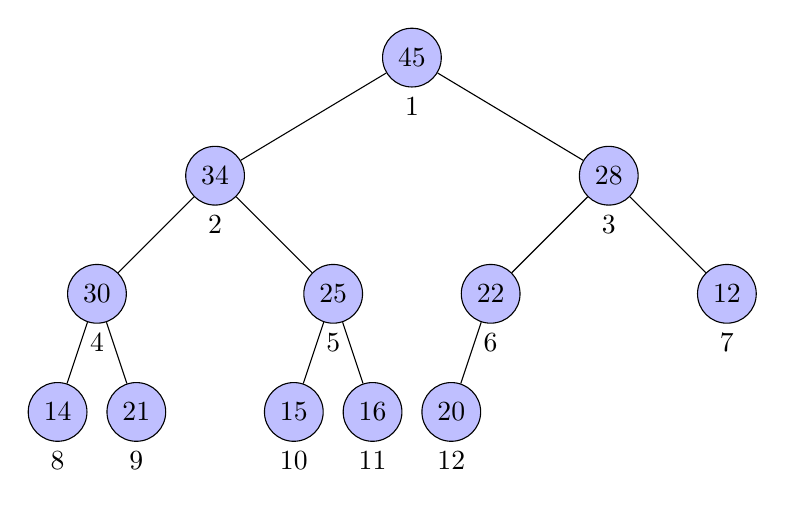
\begin{tikzpicture}
		[level 1/.style={sibling distance=5cm},
		level 2/.style={sibling distance=3cm},
		level 3/.style={sibling distance=1cm},
		mynode/.style = {shape=circle, draw, align=center, fill=blue!25!white,minimum size=.5cm}]
		\node[mynode,name=1]{45}
		child{
			node[mynode,name=2]{34}
			child{
				node[mynode,name=4]{30}
				child{
					node[mynode,name=8]{14}
				}
				child{
					node[mynode,name=9]{21}
				}
			}
			child{
				node[mynode,name=5]{25}
				child{
					node[mynode,name=10]{15}
				}
				child{
					node[mynode,name=11]{16}
				}
			}
		}
		child{
		node[mynode,name=3]{28}
			child{
				node[mynode,name=6]{22}
				child{
					node[mynode,name=12]{20}
				}
				child[mynode,missing]
			}
			child{
				node[mynode,name=7]{12}
			}
	};
\foreach \i in {1,...,12}
{
	\node[anchor=north] at (\i.south) {\i};
}
	\end{tikzpicture}
\end{center}

Quindi gli indici dell'array andranno da sinistra verso destra livello per livello:
\begin{center}
    \begin{tikzpicture}
	\def\sz{8mm}
	\tikzstyle{block} = [draw, fill=black!10, rectangle,minimum height=\sz, minimum width=\sz ];
	\tikzstyle{plain} = [draw=none,fill=none];
	\def\arr{45,34,28,30,25,22,12,14,21,15,16,20};
	\newcounter{ind};
	\setcounter{ind}{0};
	\node[plain] { $A$ };
	\foreach \item in \arr
	{
		\addtocounter{ind}{1};
		\node[block,name=\item] at (\theind*\sz,0) { \item };
		\node[plain] at (\theind*\sz,0.7) { \theind };
	}
\end{tikzpicture}
\end{center}

 Dunque \textbf{un heap può essere implementato come un array }$A$ in cui:
\begin{itemize}
	\item la radice dello heap sta nella posizione $A[0]$ dell'array.
	\item Se il nodo $i$ dello Heap sta nella posizione $i$ dell'array (cioè $A[i]$) allora:
	\begin{itemize}
		\item il figlio sinistro di $i$ sta nella posizione $2i$;
		\item il figlio destro di $i$ sta nella posizione $2i+1$;
	\end{itemize}
\end{itemize}

Dunque \textbf{un array sarà un albero heap} se soddisfa le condizioni:
\begin{eqnarray}
	 A[i]\geq A[2i]  \label{eq:heap1}\\
	A[i]\geq A[2i+1] \label{eq:heap2}
\end{eqnarray}

Da questa corrispondenza si ottiene anche che le posizioni nell'array che contengono le foglie sono quelle per cui $2i>n$, da cui $i > \frac{n}{2}$, ovvero nella \textbf{seconda metà di destra dell'array}. Più precisamente i nodi interni andranno da $1 \leq i \leq \lfloor n/2 \rfloor$, mentre le foglie da $\lfloor n/2 \rfloor \leq i \leq n$.

Un array $A$ che rappresenta un albero heap è caratterizzato dall'attributo \texttt{\textbf{heapsize}} il quale denota il numero di nodi dell'albero heap correntemente memorizzati nel vettore. Chiaramente si ha sempre:
\begin{displaymath}
	0 \leq \text{\texttt{heapsize}} \leq \text{\texttt{A.lenght}}
\end{displaymath}
Anche se ci possono essere dei numeri memorizzati in tutto l'array $A$, soltanto i numeri $A[1,\ldots,heapsize]$ sono elementi validi dell'heap. La radice dell'albero viene sempre memorizzata in $A[1]$. Se $i$ è l'indice di un nodo, gli indici del padre \textsc{Parent}$(i)$, del figlio sinistro \textsc{Left}$(i)$ e del figlio destro \textsc{Right}$(i)$ possono essere calcolati mediante le seguenti procedure:
\begin{minipage}{.3\textwidth}
	\begin{lstlisting}[caption={\textsc{Parent}(i)},language=asd]
		return  @$\lfloor \frac{n}{2}\rfloor$@
	\end{lstlisting}
\end{minipage}
\hfil
\begin{minipage}{.3\textwidth}
	\begin{lstlisting}[caption={\textsc{Left}(i)},language=asd]
		return @$2i$@
	\end{lstlisting}
\end{minipage}
\hfil
\begin{minipage}{.3\textwidth}
	\begin{lstlisting}[caption={\textsc{Right}(i)},language=asd]
		return @$2i+1$@
	\end{lstlisting}
\end{minipage}

\begin{center}
	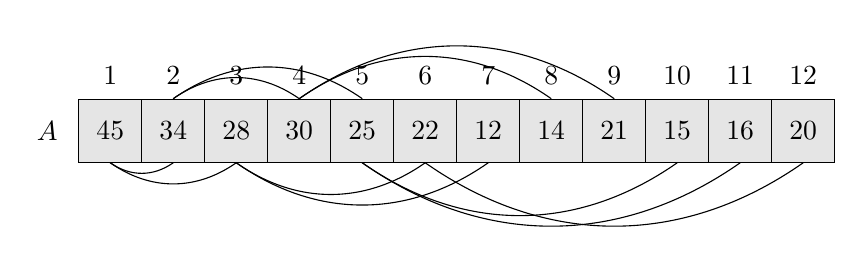
\begin{tikzpicture}
		\def\sz{8mm}
		\tikzstyle{block} = [draw, fill=black!10, rectangle,minimum height=\sz, minimum width=\sz ];
		\tikzstyle{plain} = [draw=none,fill=none];
		\def\arr{45,34,28,30,25,22,12,14,21,15,16,20};
		\setcounter{ind}{0};
		\node[plain] { $A$ };
		\foreach \item in \arr
		{
			\addtocounter{ind}{1};
			\node[block,name=\item] at (\theind*\sz,0) { \item };
			\node[plain] at (\theind*\sz,0.7) { \theind};
		}
	\draw[-] (45.south) to [bend right=35] (34.south);
	\draw[-] (45.south) to [bend right=35] (28.south);
	\draw[-] (34.north) to [bend left=35] (30.north);
	\draw[-] (34.north) to [bend left=35] (25.north);
	\draw[-] (28.south) to [bend right=35] (22.south);
	\draw[-] (28.south) to [bend right=35] (12.south);
	\draw[-] (30.north) to [bend left=35] (14.north);
	\draw[-] (30.north) to [bend left=35] (21.north);
	\draw[-] (25.south) to [bend right=35] (15.south);
	\draw[-] (25.south) to [bend right=35] (16.south);
	\draw[-] (22.south) to [bend right=35] (20.south);
	\end{tikzpicture}
\captionof{figure}{}\label{fig:heap3}
\end{center}

\subsection{L'algoritmo \textsc{Heapify}: conservare la proprietà dell'heap}
Come osservato fino a questo punto, un vettore rappresentante un albero heap gode di un ordinamento parziale dato dalle relazioni \ref{eq:heap1} e \ref{eq:heap2}. Basta osservare l'array $A$ mostrato in Figura \ref{fig:heap3} per convincersi del fatto che tale vettore non sia totalmente ordinato.

Volendo ripetere il ragionamento fatto per l'algoritmo \textsc{SelectionSort} (Algoritmo \ref{alg:selectionsort}) si potrebbe pensare di utilizzare un algoritmo \textsc{FindMax} che, dato un array $A$ e un indice $i$, restituisca l'indice $j$ del massimo elemento dell'array $A[i,\ldots,n]$. Tale algoritmo però non è sufficiente per garantire che l'array $A$ sia di nuovo un heap. Infatti, se si considera l'array $A$ mostrato in Figura \ref{fig:heap3} e si applica l'algoritmo \textsc{FindMax}$(A,1)$ si ottiene che il massimo elemento è $45$ e che si trova nella posizione $1$. Se si scambia l'elemento $45$ con l'elemento $20$ si ottiene l'array $A'$ mostrato in Figura \ref{fig:heap4} che non è un heap.

\begin{center}
	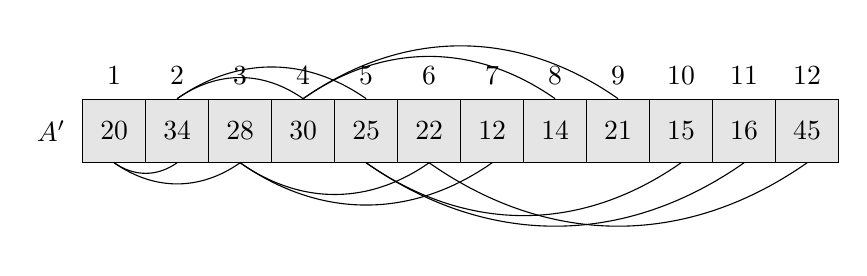
\begin{tikzpicture}
		\def\sz{8mm}
		\tikzstyle{block} = [draw, fill=black!10, rectangle,minimum height=\sz, minimum width=\sz ];
		\tikzstyle{plain} = [draw=none,fill=none];
		\def\arr{20,34,28,30,25,22,12,14,21,15,16,45};
		\setcounter{ind}{0};
		\node[plain] { $A'$ };
		\foreach \item in \arr
		{
			\addtocounter{ind}{1};
			\node[block,name=\item] at (\theind*\sz,0) { \item };
			\node[plain] at (\theind*\sz,0.7) { \theind};
		}
	\draw[-] (20.south) to [bend right=35] (34.south);
	\draw[-] (20.south) to [bend right=35] (28.south);
	\draw[-] (34.north) to [bend left=35] (30.north);
	\draw[-] (34.north) to [bend left=35] (25.north);
	\draw[-] (28.south) to [bend right=35] (22.south);
	\draw[-] (28.south) to [bend right=35] (12.south);
	\draw[-] (30.north) to [bend left=35] (14.north);
	\draw[-] (30.north) to [bend left=35] (21.north);
	\draw[-] (25.south) to [bend right=35] (15.south);
	\draw[-] (25.south) to [bend right=35] (16.south);
	\draw[-] (22.south) to [bend right=35] (45.south);
	\end{tikzpicture}
	\captionof{figure}{}\label{fig:heap4}
\end{center}
Per questo motivo, per mantenere la proprietà di heap è necessario usare l'algoritmo \textsc{Heapify} (Algoritmo \ref{alg:heapify}) che, dato un array $A$ e un indice $i$, \textbf{ripristina la proprietà di heap} nell'albero binario con radice in $i$ assumendo che i sottoalberi con radici in \textsc{Left}$(i)$ e \textsc{Right}$(i)$ siano heap e che l'unico elemento che non rispetta la proprietà di heap sia $A[i]$. L'algoritmo \textsc{Heapify} non fa altro che far ``scendere'' l'elemento $A[i]$ nell'albero fino a che l'albero con radice in $i$ non sia un heap.

\begin{example}
	Supponiamo di avere il vettore: $A= [16,4,10,14,7,9,3,2,8,1]$. La Figura \ref{fig:heapify} mostra l'azione dell'algoritmo \textsc{Heapify}.
\end{example}

\begin{center}
	\begin{minipage}{\textwidth}
		\centering
		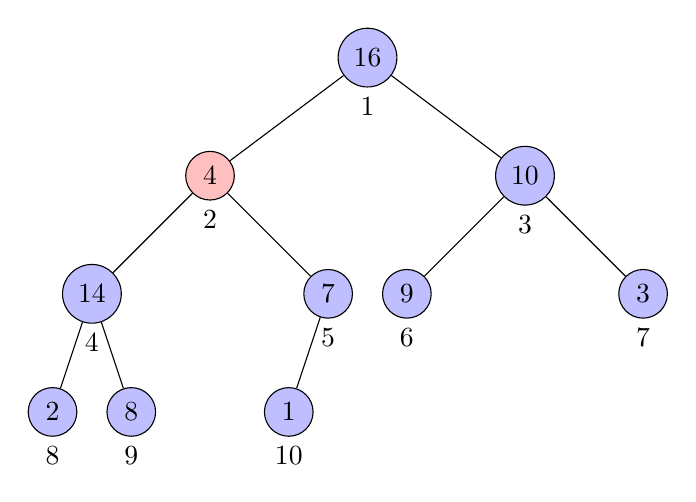
\begin{tikzpicture}
			[mynode/.style={circle,draw,fill=blue!25!white,minimum size=0.5cm},
			level 1/.style={sibling distance=4cm},
			level 2/.style={sibling distance=3cm},
			level 3/.style={sibling distance=1cm},]
			\node[mynode,name=1]{16}
			child
			{
				node[mynode,name=2,fill=red!25!white]{4}
				child
				{
					node[mynode,name=4]{14}
						child
						{
							node[mynode,name=8]{2}
						}
						child
						{
							node[mynode,name=9]{8}	
						}
				}
					child
					{
						node[mynode,name=5]{7}
							child
							{
								node[mynode,name=10]{1}
							}
							child[missing]
					}
			}
			child
			{
				node[mynode,name=3]{10}
				child
				{
					node[mynode,name=6]{9}
				}
				child
				{
					node[mynode,name=7]{3}
				}
			};
		\foreach \i in {1,...,10}
		{
			\node[anchor=north] at (\i.south) {\i};
		}
		\end{tikzpicture}
	\captionof{figure}{La configurazione iniziale, con $A[2]$ nel nodo $i=2$ che viola le proprietà di heap.}
	\end{minipage}
	\\
	\begin{minipage}{\textwidth}
		\centering
		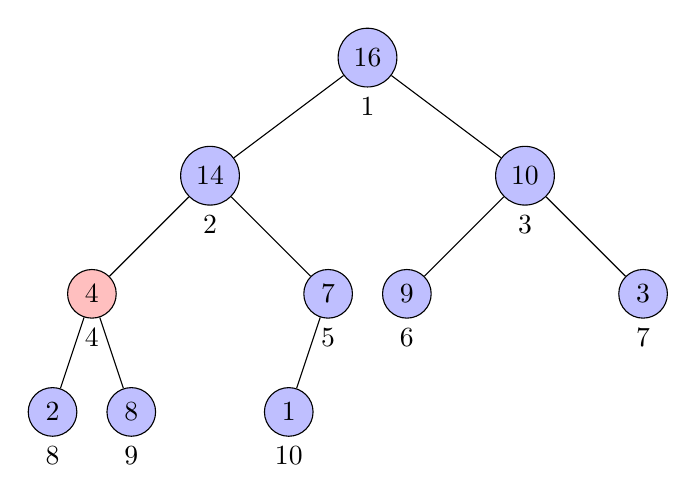
\begin{tikzpicture}
			[mynode/.style={circle,draw,fill=blue!25!white,minimum size=0.5cm},
			level 1/.style={sibling distance=4cm},
			level 2/.style={sibling distance=3cm},
			level 3/.style={sibling distance=1cm},]
			\node[mynode,name=1]{16}
			child
			{
				node[mynode,name=2]{14}
				child
				{
					node[mynode,name=4,fill=red!25!white]{4}
					child
					{
						node[mynode,name=8]{2}
					}
					child
					{
						node[mynode,name=9]{8}	
					}
				}
				child
				{
					node[mynode,name=5]{7}
					child
					{
						node[mynode,name=10]{1}
					}
					child[missing]
				}
			}
			child
			{
				node[mynode,name=3]{10}
				child
				{
					node[mynode,name=6]{9}
				}
				child
				{
					node[mynode,name=7]{3}
				}
			};
			\foreach \i in {1,...,10}
			{
				\node[anchor=north] at (\i.south) {\i};
			}
		\end{tikzpicture}
	\captionof{figure}{Le proprietà di heap vengono ripristinate nel nodo $2$ scambiando $A[2]$ con $A[4]$; ma questo distrugge la proprietà di heap nel nodo 4, sarà necessario richiamare l'algoritmo \textsc{Heapify}$(A,4)$.}
	\end{minipage}
	\\
	\begin{minipage}{\textwidth}
		\centering
			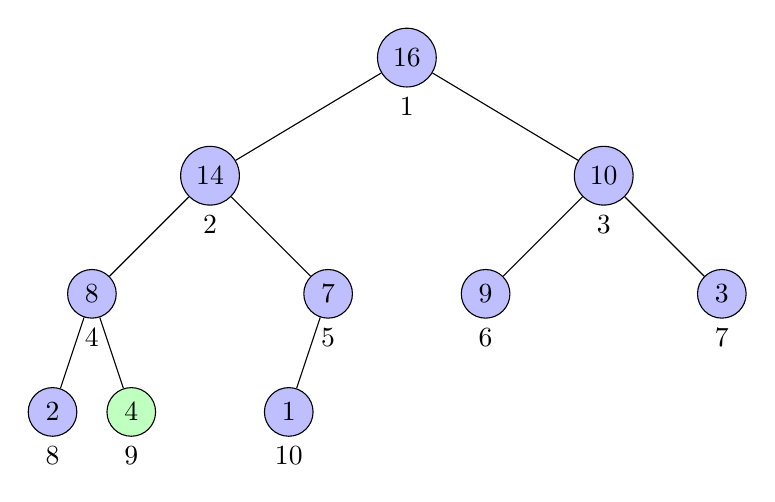
\begin{tikzpicture}
		[mynode/.style={circle,draw,fill=blue!25!white,minimum size=0.5cm},
		level 1/.style={sibling distance=5cm},
		level 2/.style={sibling distance=3cm},
		level 3/.style={sibling distance=1cm},]
		\node[mynode,name=1]{16}
		child
		{
			node[mynode,name=2]{14}
			child
			{
				node[mynode,name=4]{8}
				child
				{
					node[mynode,name=8]{2}
				}
				child
				{
					node[mynode,name=9,fill=green!25!white]{4}	
				}
			}
			child
			{
				node[mynode,name=5]{7}
				child
				{
					node[mynode,name=10]{1}
				}
				child[missing]
			}
		}
		child
		{
			node[mynode,name=3]{10}
			child
			{
				node[mynode,name=6]{9}
			}
			child
			{
				node[mynode,name=7]{3}
			}
		};
		\foreach \i in {1,...,10}
		{
			\node[anchor=north] at (\i.south) {\i};
		}
	\end{tikzpicture}
		\captionof{figure}{La chiamata ricorsiva \textsc{Heapify}$(A,4)$ scambia $A[4]$ con $A[9]$, il nodo $4$ è sistemato e la chiamata \textsc{Heapify}$(A,9)$ non apporta modifiche in quanto le foglie rispettano sempre la proprietà heap.}\label{fig:heapify}
	\end{minipage}
\end{center}

Ad ogni passo, viene determinato il più grande tra $A[i]$, $A[2i]$ e $A[2i+1]$; il suo indice viene memorizzato nella variabile \texttt{max}. Se $A[i]$ è più grande, allora il sottoalbero con radice nel nodo $i$ è un heap e la procedura termina. Altrimenti, uno dei due figli ha l'elemento più grande e $A[i]$ viene scambiato con $A[max]$; in questo modo, il nodo $i$ e i suoi figli soddisfano la proprietà di heap. Il nodo con indice $max$, però, adesso ha il valore originale $A[i]$ e, quindi, il sottoalbero con radice in $max$ potrebbe violare la proprietà di heap. Di conseguenza, deve essere richiamata ricorsivamente la procedura \textsc{Heapify}$(A,max)$ per quel sottoalbero.

\begin{lstlisting}[language=asd,caption={\textsc{Heapify}(A,i)},label=alg:heapify]
	Sx = Left(i)
	Dx = Right(i)
	if (Sx <= heapsize && A[i]<A[Sx]) then
	max = Sx
	else
	max = i
	if (Dx <= heapsize && A[max] < A[Dx]) then
	max = Dx
	if (max @$\neq$@ i) then
	Swap(A,i,max)
	Heapify(A,max)
\end{lstlisting}

Il tempo di esecuzione di \textsc{Heapify} in un sottoalbero di dimensione $n$  con radice in un nodo $i$ è pari al tempo $\Theta(1)$ per sistemare le relazioni fra gli elementi, più il tempo per eseguire \textsc{Heapify} in un sottoalbero con radice in uno dei figli del nodo $i$. Dunque si può affermare che \textsc{Heapify} ha un tempo di esecuzione pari a:
\begin{equation}T_{Heapify}(n) = O(\log n)\end{equation}

L'algoritmo \ref{alg:heapify} non funziona per sequenze che non siano  heap. Infatti, se così fosse si potrebbe usare \textsc{Heapify} per cercare il massimo di una sequenza in un tempo minore di $\Theta(n)$.

\subsection{Trasformare un array in un heap: l'algoritmo \textsc{Costruisci-Heap}}

È possibile utilizzare l'Algoritmo \textsc{Heapify} dal basso verso l'alto per convertire un array $A[1,\ldots,n]$ in un heap:
\begin{itemize}
	\item  Ovviamente una foglia rispetta sempre le proprietà degli heap,  quindi gli ultimi $\lceil \frac{n}{2} \rceil$ elementi dell'array sono già degli heap. Prendendo i padri delle foglie si può applicare \textsc{Heapify} poiché tutti i loro sottoalberi rispettano la proprietà necessaria.
	\item È sufficiente inserire nello heap solo i primi $\lfloor \frac{n}{2} \rfloor$ elementi, utilizzando \textsc{Heapify} per ripristinare la terza condizione degli heap sul sottoalbero del nuovo elemento.
\end{itemize}

Si ha quindi l'Algoritmo \textsc{Costruisci-Heap} (Algoritmo \ref{alg:costruisciheap}).

\begin{lstlisting}[language=asd,caption={\textsc{Costruisci-Heap}(A,n)},label=alg:costruisciheap]
heapsize = n
for(i= @$\lfloor n/2 \rfloor$@ down to 1 ) do
	Heapify(A,i)
\end{lstlisting}

\begin{example}
	Supponiamo di voler costruire un albero heap a partire dall'array $A=[4,1,3,2,16,9,10,14,8,7]$. La Figura \ref{fig:costruisci-heap} mostra il funzionamento dell'Algoritmo \ref{alg:costruisciheap}.
\end{example}

\begin{center}	
\begin{minipage}{.45\textwidth}
	\centering
		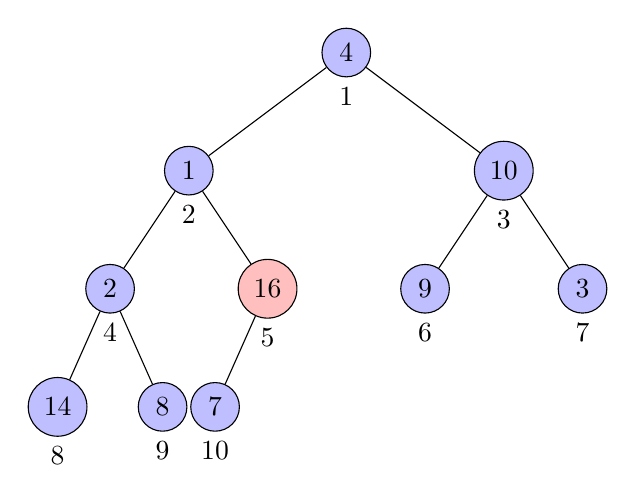
\begin{tikzpicture}
		[mynode/.style={circle,draw,fill=blue!25!white,minimum size=0.5cm},
			level/.style={sibling distance=40mm/#1}]
		\node[mynode,name=1]{4}
		child
		{
			node[mynode,name=2]{1}
			child
			{
				node[mynode,name=4]{2}
				child
				{
					node[mynode,name=8]{14}
				}
				child
				{
					node[mynode,name=9]{8}
				}
			}
			child
			{
				node[mynode,name=5,fill=red!25!white]{16}
				child
				{
					node[mynode,name=10]{7}	
				}
				child[missing]
			}
		}
		child
		{
			node[mynode,name=3]{10}
			child
			{
				node[mynode,name=6]{9}
			}
			child 
			{
				node[mynode,name=7]{3}
			}
		};
	\foreach \i in {1,...,10}
	{
		\node[anchor=north] at (\i.south) {\i};
	}
\end{tikzpicture}
\captionof{figure}{Albero binario rappresentato dall'array $A$, l'indice $i$ punta a $\lfloor 10/2 \rfloor =5 $ prima della chiamata a \textsc{Heapify}$(A,5)$.}
\end{minipage}
\hfil
\begin{minipage}{.45\textwidth}
	\centering
			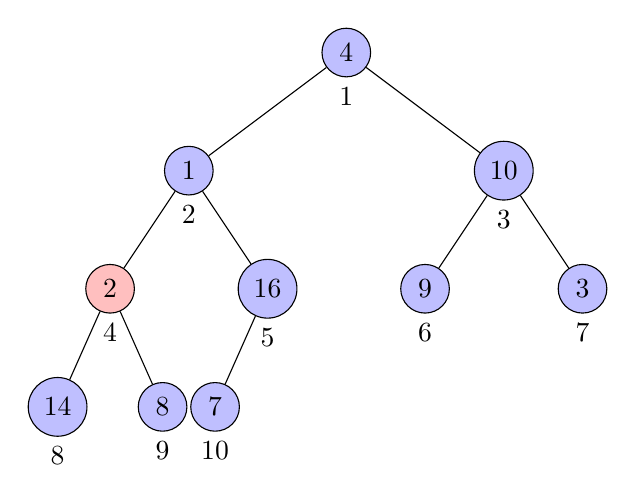
\begin{tikzpicture}
		[mynode/.style={circle,draw,fill=blue!25!white,minimum size=0.5cm},
		level/.style={sibling distance=40mm/#1}]
		\node[mynode,name=1]{4}
		child
		{
			node[mynode,name=2]{1}
			child
			{
				node[mynode,name=4,fill=red!25!white]{2}
				child
				{
					node[mynode,name=8]{14}
				}
				child
				{
					node[mynode,name=9]{8}
				}
			}
			child
			{
				node[mynode,name=5]{16}
				child
				{
					node[mynode,name=10]{7}	
				}
				child[missing]
			}
		}
		child
		{
			node[mynode,name=3]{10}
			child
			{
				node[mynode,name=6]{9}
			}
			child 
			{
				node[mynode,name=7]{3}
			}
		};
		\foreach \i in {1,...,10}
		{
			\node[anchor=north] at (\i.south) {\i};
		}
	\end{tikzpicture}
\captionof{figure}{Struttura dati risultante dopo \textsc{Heapify}$(A,5)$. L'indice $i$ per l'iterazione successiva fa riferimento al nodo 4.}
\end{minipage}\\
\begin{minipage}{.45\textwidth}
	\centering
		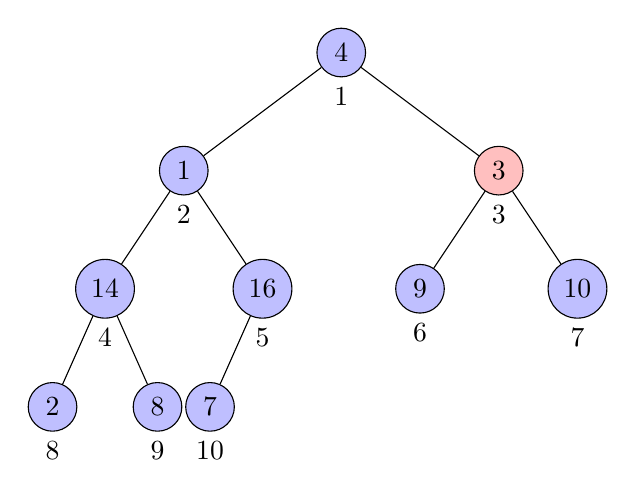
\begin{tikzpicture}
		[mynode/.style={circle,draw,fill=blue!25!white,minimum size=0.5cm},
		level/.style={sibling distance=40mm/#1}]
		\node[mynode,name=1]{4}
		child
		{
			node[mynode,name=2]{1}
			child
			{
				node[mynode,name=4]{14}
				child
				{
					node[mynode,name=8]{2}
				}
				child
				{
					node[mynode,name=9]{8}
				}
			}
			child
			{
				node[mynode,name=5]{16}
				child
				{
					node[mynode,name=10]{7}	
				}
				child[missing]
			}
		}
		child
		{
			node[mynode,name=3,fill=red!25!white]{3}
			child
			{
				node[mynode,name=6]{9}
			}
			child 
			{
				node[mynode,name=7]{10}
			}
		};
		\foreach \i in {1,...,10}
		{
			\node[anchor=north] at (\i.south) {\i};
		}
	\end{tikzpicture}
\end{minipage} \hfil
\begin{minipage}{.45\textwidth}
	\centering
	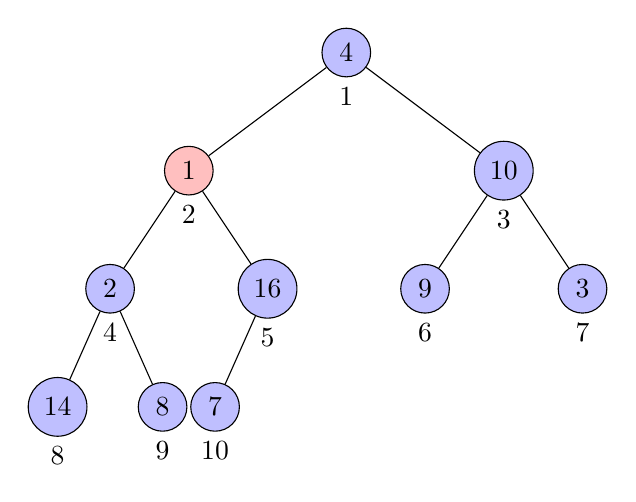
\begin{tikzpicture}
		[mynode/.style={circle,draw,fill=blue!25!white,minimum size=0.5cm},
		level/.style={sibling distance=40mm/#1}]
		\node[mynode,name=1]{4}
		child
		{
			node[mynode,name=2,fill=red!25!white]{1}
			child
			{
				node[mynode,name=4]{2}
				child
				{
					node[mynode,name=8]{14}
				}
				child
				{
					node[mynode,name=9]{8}
				}
			}
			child
			{
				node[mynode,name=5]{16}
				child
				{
					node[mynode,name=10]{7}	
				}
				child[missing]
			}
		}
		child
		{
			node[mynode,name=3]{10}
			child
			{
				node[mynode,name=6]{9}
			}
			child 
			{
				node[mynode,name=7]{3}
			}
		};
		\foreach \i in {1,...,10}
		{
			\node[anchor=north] at (\i.south) {\i};
		}
	\end{tikzpicture}
\end{minipage}\\
\begin{minipage}{.45\textwidth}
	\centering
	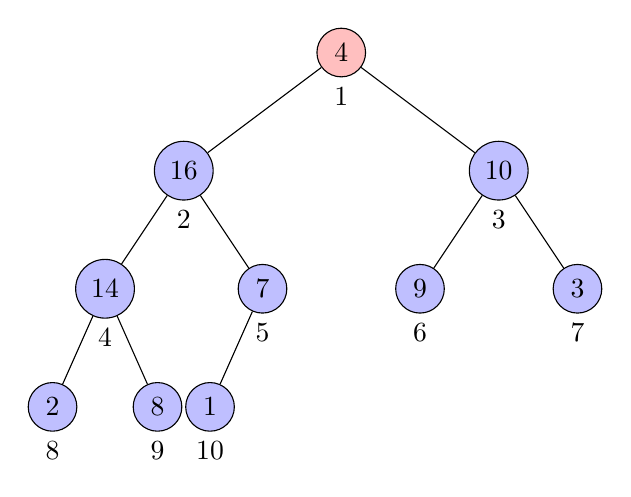
\begin{tikzpicture}
		[mynode/.style={circle,draw,fill=blue!25!white,minimum size=0.5cm},
		level/.style={sibling distance=40mm/#1}]
		\node[mynode,name=1,fill=red!25!white]{4}
		child
		{
			node[mynode,name=2]{16}
			child
			{
				node[mynode,name=4]{14}
				child
				{
					node[mynode,name=8]{2}
				}
				child
				{
					node[mynode,name=9]{8}
				}
			}
			child
			{
				node[mynode,name=5]{7}
				child
				{
					node[mynode,name=10]{1}	
				}
				child[missing]
			}
		}
		child
		{
			node[mynode,name=3]{10}
			child
			{
				node[mynode,name=6]{9}
			}
			child 
			{
				node[mynode,name=7]{3}
			}
		};
		\foreach \i in {1,...,10}
		{
			\node[anchor=north] at (\i.south) {\i};
		}
	\end{tikzpicture}
\end{minipage} \hfil
\begin{minipage}{.45\textwidth}
	\centering
	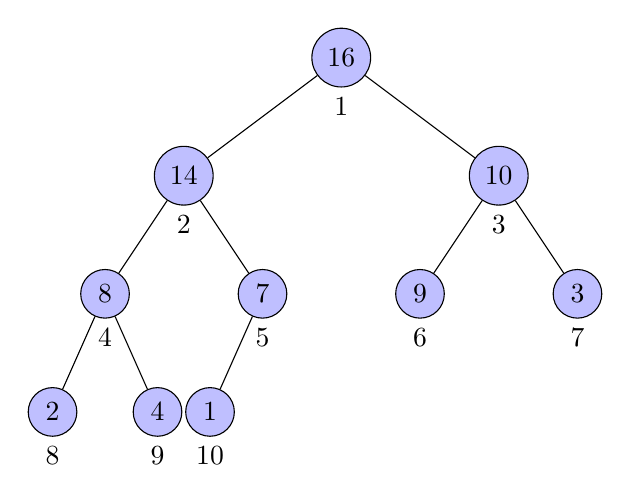
\begin{tikzpicture}
		[mynode/.style={circle,draw,fill=blue!25!white,minimum size=0.5cm},
		level/.style={sibling distance=40mm/#1}]
		\node[mynode,name=1]{16}
		child
		{
			node[mynode,name=2]{14}
			child
			{
				node[mynode,name=4]{8}
				child
				{
					node[mynode,name=8]{2}
				}
				child
				{
					node[mynode,name=9]{4}
				}
			}
			child
			{
				node[mynode,name=5]{7}
				child
				{
					node[mynode,name=10]{1}	
				}
				child[missing]
			}
		}
		child
		{
			node[mynode,name=3]{10}
			child
			{
				node[mynode,name=6]{9}
			}
			child 
			{
				node[mynode,name=7]{3}
			}
		};
		\foreach \i in {1,...,10}
		{
			\node[anchor=north] at (\i.south) {\i};
		}
	\end{tikzpicture}
\captionof{figure}{Heap finale}
\end{minipage}
\captionof{figure}{}\label{fig:costruisci-heap}
\end{center}

Ogni chiamata di \textsc{Costruisci-Heap} costa un tempo $O(\log n)$ e ci sono $O(n)$ di queste chiamate. Quindi, il tempo di esecuzione sarà $O(n \log n)$. Questo limite superiore, sebbene corretto, non è asintoticamente stretto.

Possiamo ottenere un limite più stretto osservando che il tempo per eseguire \textsc{Heapify} (Algoritmo \ref{alg:heapify}) in un nodo varia con l'altezza del nodo nell'albero, e le altezze della maggior parte dei nodi sono piccole. L'analisi più rigorosa si basa sulla proprietà che un heap di $n$ elementi ha un'altezza $\lfloor n/2 \rfloor$ e, per ogni $h$, al massimo $\lceil n/2^{h+1} \rceil$ nodi di altezza $h$. Il tempo richiesto dalla procedura \textsc{Heapify} quando viene chiamata per un nodo di altezza $h$ è $O(h)$, quindi possiamo dire che il costo totale di \textsc{Costruisci-Heap} è limitato superiormente da:
\begin{displaymath}
	\sum_{h=0}^{\lfloor \log n \rfloor} \lceil \frac{n}{2^{h+1}} \rceil O(h)= O\Bigl(n \sum_{h=0}^{\lfloor \log n \rfloor} \frac{h}{2^{h}} \Bigl)
\end{displaymath}


\begin{propbox}
	Derivando entrambi i lati della serie geometrica infinita e moltiplicando per $x$, si ha, 	per $|x|<1$:
	\begin{equation}\label{sommatoria:integrale}
		\sum_{k=0}^{\infty} kx^{k} = \frac{x}{{(1-x)}^{2}}
	\end{equation}
\end{propbox}

L'ultima sommatoria può essere calcolata ponendo $x=1/2$ nella formula \ref{sommatoria:integrale}:
\begin{displaymath}
	\sum_{h=0}^{\infty} \frac{h}{2^{h}} = \frac{1/2}{(1-1/2)^{2}}=2
\end{displaymath}

Quindi, il tempo di esecuzione di \textsc{Costruisci-Heap} può essere limitato così:
\begin{equation}
	O\Bigl(n \sum_{h=0}^{\lfloor \log n \rfloor} \frac{h}{2^{h}} \Bigl) = O\Bigl(n \sum_{h=0}^{\infty} \frac{h}{2^{h}}\Bigl)=O(n)
\end{equation}

Dunque possiamo costruire un heap da un array non ordinato in tempo lineare.

\subsection{L'algoritmo \textsc{HeapSort}}
Come anticipato, l'algoritmo \textsc{HeapSort} è una variazione di \textsc{SelectionSort} in cui la ricerca dell'elemento massimo è facilitata dal mantenimento della sequenza in uno heap.
L'algoritmo inizia utilizzando \textsc{Costruisci-Heap} per costruire un heap nell'array di input $A[1..n]$, dove $n$ è la lunghezza di $A$.

Poiché l'elemento più grande dell'array è memorizzato nella radice $A[1]$, esso può essere inserito nella sua posizione finale corretta scambiandolo con $A[n]$. Se adesso ``togliamo'' il nodo $n$ dall'heap (diminuendo la variabile \textit{heapsize}), notiamo che i figli della radice restano degli alberi heap, ma la nuova radice potrebbe violare la proprietà dell'heap. Per ripristinare questa proprietà, tuttavia, basta una chiamata di \textsc{Heapify}$(A,1)$ (Algoritmo \ref{alg:heapify}), che lascia un heap in $A[1,..,n-1]$. L'algoritmo \textsc{HeapSort} poi ripete questo processo per il sottoalbero heap di dimensione $n-1$ e così via fino ad un heap di dimensione due.

\begin{lstlisting}[caption={\textsc{HeapSort}(A)},label=alg:heapsort,language=asd]
	Costruisci-Heap(A)
	for (i = n down to 2) do
		Swap(A,1,i)
		heapsize = heapsize -1
		Heapify(A,1)
\end{lstlisting}

La procedura \textsc{HeapSort} (Algoritmo \ref{alg:heapsort}) impiega un tempo $O(n \log n)$, in quanto la chiamata di \textsc{Costruisci-Heap} impiega $O(n)$ e ciascuna delle $n-1$ chiamate di \textsc{Heapify} impiega un tempo $O(n \log n)$.

\section{Quick Sort}
L'Algoritmo\textsc{QuickSort}, come \textsc{MergeSort}, è basato sul paradigma divide et impera. Questi sono i tre passi del processo divide et impera per ordinare un generico sottoarray $A[p..r]$.
\begin{enumerate}
	\item \textbf{Divide:} partizionare l'array $A[p..r]$ in due sottoarray $A[p..q-1]$ e $A[q+1..r]$ (eventualmente vuoti) tali che ogni elemento di $A[p..q-1]$ sia minore o uguale ad $A[q]$ che, a sua volta, è minore o uguale ad ogni elemento di $A[q+1..r]$. Calcolare l'indice $q$ come parte di questa procedura di partizionamento.
	\item \textbf{Impera:} ordinare i due sottoarray $A[p..q-1]$ e $A[q+1..r]$ chiamando ricorsivamente \textsc{QuickSort}.
	\item \textbf{Combina:} poiché i sottoarray sono già ordinati, non occorre alcun lavoro per combinarli: l'intero array $A[p..r]$ è già ordinato.
\end{enumerate}

\begin{lstlisting}[caption={\textsc{QuickSort}(A,p,r)},label={alg:quicksort},language=asd]
		if p<r
			q=Partiziona(A,p,r)
			QuickSort(A,p,q)
			QuickSort(A,q+1,r)
\end{lstlisting}
Per ordinare un intero array $A$ di lunghezza $n$, la chiamata iniziale è \textsc{QuickSort}$(A,1,n)$.

\begin{osservation}
	L'algoritmo \textsc{MergeSort} decompone l'array in maniera aritmetica dividendo a metà iterativamente l'array in sottoarray. Così facendo la decomposizione in sottoprobremi risulta più semplice a discapito della fase fusione che è più complessa. L'algoritmo \textsc{QuickSort} decompone in modo ``intelligente'' (pagando di più in termini computazionali) in modo tale da semplificare la fusione dei sottoarray così ottenuti.
\end{osservation}

L'algoritmo \textsc{QuickSort} (Algoritmo \ref{alg:quicksort}) è corretto se valgono le seguenti proprietà:
\begin{enumerate}
	\item La partizione $A[p..q]$ è strettamente minore della sequenza $A[p..r]$.
	\item La partizione $A[q+1..r]$ è strettamente minore della sequenza $A[p..r]$.
	\item Al termine di \textsc{Partiziona}$(A,p,r)$ deve valere:
	\begin{displaymath}
		\forall \ i \in [p,q] \Bigl( \forall j \in [q+1,r] \bigl( A[i] \leq A[j]\bigr)\Bigr)
	\end{displaymath}
che esprime il fatto che ogni elemento di una sottopartizione sinistra deve essere sempre minore od uguale ad un elemento di una sottopartizione di destra.
\end{enumerate}

Le proprietà 1 e 2 possono essere sintetizzate nella proprietà:
\begin{equation}\label{prop:quicksortpartiziona}
	p \leq q < r
\end{equation}

Se questa proprietà non fosse soddisfatta l'algoritmo non funzionerebbe. Infatti è importante escludere i valori $q=p-1$ e $q=r$ per i seguenti motivi: se $q=p-1$ allora \textsc{QuickSort}$(A,p,p-1)$ starebbe passando una istanza vuota, quindi non farebbe nulla. Il problema nasce con la sequenza a destra che andrà da $p$ ad $r$, andando conseguentemente in loop. In modo analogo si ha per $q=r$.

\subsection{Partizionare l'array: l'algoritmo \textsc{Partiziona}}
L'elemento chiave dell'algoritmo \ref{alg:quicksort} è la procedura \textsc{Partiziona} che riarrangia il sottoarray $A[p..r]$ sul posto. I passi fondamentali nell'algoritmo di partizionamento (Algoritmo \ref{alg:partiziona}) sono:
\begin{enumerate}
	\item Estendere le due partizioni verso l'interno finché non si incontra una coppia non correttamente disposta;
	\item Finché le due partizioni non si sono incrociate ($i \geq j$):
	\begin{enumerate}
		\item Scambiare le coppie non correttamente disposte;
		\item Estendere ancora le due partizioni verso l'interno finché non si trova un'altra coppia non correttamente disposta.
	\end{enumerate}
\end{enumerate}
Quando viene chiamato l'algoritmo siamo certi che valga la condizione $p<r$. L'algoritmo \textsc{Partiziona} seleziona un valore $x \in A$, detto \textbf{pivot} e inserisce nella partizione sinistra gli elementi $a_{i} \leq x$ e nella partizione a destra gli elementi $a_{i}\geq x$ (non possiamo mettere il minore stretto perché l'algoritmo deve funzionare per tutte le istanze). 

\marker{yellow!50}{yellow!20!black}{Nel nostro algoritmo \textbf{il pivot è preso nel primo elemento della sottosequenza} ma, in realtà, è possibile prendere qualsiasi elemento dell'array come pivot, a patto che venga messo in prima posizione successivamente.}

\begin{center}
	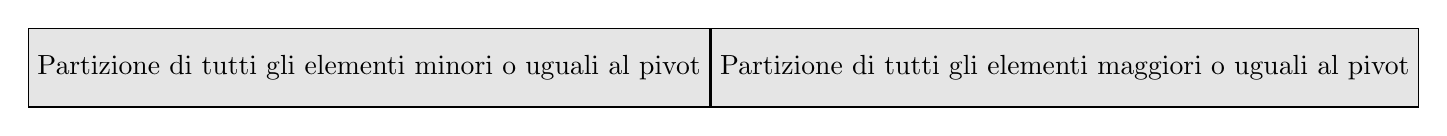
\begin{tikzpicture}
		\node[draw,fill=black!10,rectangle,name=1,minimum height=1cm,minimum width=4cm]{Partizione di tutti gli elementi minori o uguali al pivot};
		\node[draw,fill=black!10,rectangle,anchor=west,minimum height=1cm,minimum width=4cm]at(1.east){Partizione di tutti gli elementi maggiori o uguali al pivot};
	\end{tikzpicture}
\end{center}

Per scorrere la sequenza si fa uso di due indici:
\begin{enumerate}
	\item Un indice $i$ che partirà da sinistra per essere incrementato fino a quando non trova un valore $y\geq x$
	\item Un indice $j$ che partendo da destra viene decrementato fino a quando non trova un valore $z \leq x$
\end{enumerate}
Una volta fermati gli indici si effettua uno scambio e si ripete il processo fino a quando gli indici non si incrociano: vale cioè la condizione $i \geq j$.

\begin{lstlisting}[caption={\textsc{Partiziona}(A,p,r)},label=alg:partiziona,language=asd]
	x=A[p]
	j=r+1
	i=p-1
	repeat
		repeat
			j=j-1
		until (A[j] @$\leq$@ x)

		repeat
			i=i+1
		until (A[i]@$\geq$@ x)

		if (i<j)
			Swap(A,i,j)
	until (i	@$\geq$@ j)
	return j
\end{lstlisting}

\begin{example}
	Consideriamo l'array $A=[2,8,7,1,3,5,6,4]$ e osserviamo l'esecuzione dell'algoritmo \textsc{QuickSort}$(A,1,8)$.
\end{example}

La procedura di ordinamento inizia con l'invocazione di \textsc{QuickSort}$(A,1,8)$ il quale chiama \textsc{Partiziona}$(A,1,8)$. Il pivot (evidenziato in verde) viene selezionato nella posizione $A[1]$ mentre gli indici $i,j$ assumono i valori $i=0$ e $j=9$:
	\begin{center}
		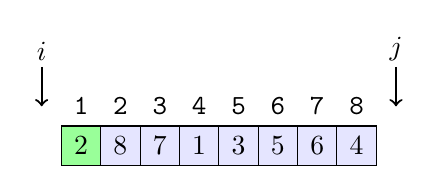
\begin{tikzpicture}
		[box/.style={rectangle,draw=black, fill=blue!10!white,minimum size=.5cm},
		plain/.style={draw=none,fill=none,font=\ttfamily}
		]
		\node[box,fill=green!40] at (0.5,0){2};
		\node[box] at (1,0){8};
		\node[box] at (1.5,0){7};
		\node[box] at (2,0){1};
		\node[box] at (2.5,0){3};
		\node[box] at (3,0){5};
		\node[box] at (3.5,0){6};
		\node[box] at (4,0){4};

\node[plain] at (.5,0.5){1};
\node[plain] at (1,0.5){2};
\node[plain] at (1.5,0.5){3};
\node[plain] at (2,0.5){4};
\node[plain] at (2.5,0.5){5};
\node[plain] at (3,0.5){6};
\node[plain] at (3.5,0.5){7};
\node[plain] at (4,0.5){8};
		\draw[->, thick] (0,1) --  node[above,yshift=2mm]{$i$} (0,.5);
		\draw[->, thick] (4.5,1) --  node[above,yshift=2mm]{$j$} (4.5,.5);
	\end{tikzpicture}
	\end{center}


Alla prima iterazione del \texttt{repeat-until} le variabili $i$ e $j$ assumono i valori $i=1$ e $j=4$ e vengono scambiati gli elementi $A[1]=2$ e $A[4]=1$:

\begin{center}
	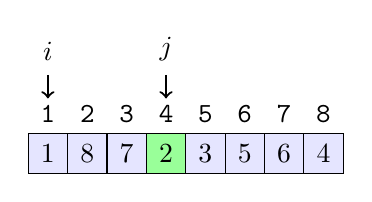
\begin{tikzpicture}
[	box/.style={rectangle,draw=black, fill=blue!10!white,minimum size=.5cm},
plain/.style={draw=none,fill=none,font=\ttfamily}
]
\node[box] at (.5,0){1};
\node[box] at (1,0){8};
\node[box] at (1.5,0){7};
\node[box,fill=green!40] at (2,0){2};
\node[box] at (2.5,0){3};
\node[box] at (3,0){5};
\node[box] at (3.5,0){6};
\node[box] at (4,0){4};

\node[plain] at (.5,0.5){1};
\node[plain] at (1,0.5){2};
\node[plain] at (1.5,0.5){3};
\node[plain] at (2,0.5){4};
\node[plain] at (2.5,0.5){5};
\node[plain] at (3,0.5){6};
\node[plain] at (3.5,0.5){7};
\node[plain] at (4,0.5){8};

\draw[->, thick] (.5,1) --  node[above,yshift=2mm]{$i$} (.5,.7);
\draw[->, thick] (2,1) --  node[above,yshift=2mm]{$j$} (2,.7);
\end{tikzpicture}
\end{center}


Nella ripetizione successiva gli indici assumono valori $i=2$ e $j=1$ e la \textsc{Partiziona} restituisce $q=1$. A questo punto viene invocato \textsc{QuickSort}$(A,1,1)$ che termina immediatamente e \textsc{QuickSort}$(A,2,8)$ il quale invoca \textsc{Partiziona}$(A,2,8)$. Il pivot è $A[2]=8$, gli indici $i,j$ inizialmente valgono $i=1$ e $j=9$:
	
\begin{center}
		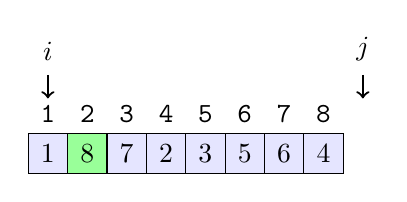
\begin{tikzpicture}
			[	box/.style={rectangle,draw=black, fill=blue!10!white,minimum size=.5cm},
			plain/.style={draw=none,fill=none,font=\ttfamily}
			]
			\node[box] at (.5,0){1};
			\node[box,fill=green!40] at (1,0){8};
			\node[box] at (1.5,0) {7};
			\node[box] at (2,0) {2};
			\node[box] at (2.5,0) {3};
			\node[box] at (3,0) {5};
			\node[box] at (3.5,0) {6};
			\node[box] at (4,0) {4};

			\node[plain] at (0.5,0.5) {1};
			\node[plain] at (1,0.5){2};
			\node[plain] at (1.5,0.5){3};
			\node[plain] at (2,0.5){4};
			\node[plain] at (2.5,0.5){5};
			\node[plain] at (3,0.5){6};
			\node[plain] at (3.5,0.5){7};
			\node[plain] at (4,0.5){8};
			\draw[->, thick] (.5,1) --  node[above,yshift=2mm]{$i$} (.5,.7);
			\draw[->, thick] (4.5,1) --  node[above,yshift=2mm]{$j$} (4.5,.7);
		\end{tikzpicture}
\end{center}
	
Dopo la prima ripetizione gli indici assumono i valori $i=2$ e $j=8$ e si scambiano i valori $A[2]=8$ e $A[8]=4$

\begin{center}
	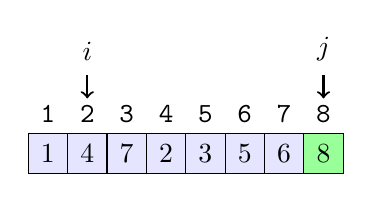
\begin{tikzpicture}
	[	box/.style={rectangle,draw=black, fill=blue!10!white,minimum size=.5cm},
	plain/.style={draw=none,fill=none,font=\ttfamily}
	]
	\node[box] at (.5,0){1};
	\node[box] at (1,0){4};
	\node[box] at (1.5,0){7};
	\node[box] at (2,0){2};
	\node[box] at (2.5,0){3};
	\node[box] at (3,0){5};
	\node[box] at (3.5,0){6};
	\node[box,fill=green!40] at (4,0){8};

\node[plain] at (.5,0.5){1};
\node[plain] at (1,0.5){2};
\node[plain] at (1.5,0.5){3};
\node[plain] at (2,0.5){4};
\node[plain] at (2.5,0.5){5};
\node[plain] at (3,0.5){6};
\node[plain] at (3.5,0.5){7};
\node[plain] at (4,0.5){8};
	\draw[->, thick] (1,1) --  node[above,yshift=2mm]{$i$} (1,.7);
	\draw[->, thick] (4,1) --  node[above,yshift=2mm]{$j$} (4,.7);
\end{tikzpicture}
\end{center}

Nella ripetizione successiva gli indici assumono i valori $i=8$ e $j=7$ e la procedura restituisce il valore $j=7$. Ottenuto $q=7$ si effettuano le chiamate ricorsive \textsc{QuickSort}$(A,2,7)$ e \textsc{QuickSort}$(A,8,8)$ la quale termina immediatamente. \textsc{QuickSort}$(A,2,7)$ attiva \textsc{Partiziona}$(A,2,7)$. Il pivot è $A[2]=4$, gli indici iniziali sono $i=1,j=8$.

\begin{center}
		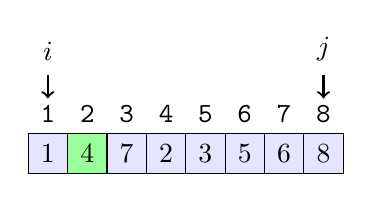
\begin{tikzpicture}
		[	box/.style={rectangle,draw=black, fill=blue!10!white,minimum size=.5cm},
		plain/.style={draw=none,fill=none,font=\ttfamily}
		]
		\node[box] at (.5,0){1};
		\node[box,fill=green!40] at (1,0){4};
		\node[box] at (1.5,0){7};
		\node[box] at (2,0){2};
		\node[box] at (2.5,0){3};
		\node[box] at (3,0){5};
		\node[box] at (3.5,0){6};
		\node[box] at (4,0){8};

\node[plain] at (.5,0.5){1};
\node[plain] at (1,0.5){2};
\node[plain] at (1.5,0.5){3};
\node[plain] at (2,0.5){4};
\node[plain] at (2.5,0.5){5};
\node[plain] at (3,0.5){6};
\node[plain] at (3.5,0.5){7};
\node[plain] at (4,0.5){8};
		\draw[->, thick] (.5,1) --  node[above,yshift=2mm]{$i$} (.5,.7);
		\draw[->, thick] (4,1) --  node[above,yshift=2mm]{$j$} (4,.7);
	\end{tikzpicture}
\end{center}

Alla prima ripetizione del \texttt{repeat-until} gli indici assumono i valori $i=2$ e $j=5$ e si effettua lo swap tra $A[2]=4$ e $A[5]=3$.
\begin{center}
		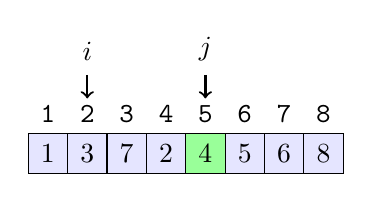
\begin{tikzpicture}
	[	box/.style={rectangle,draw=black, fill=blue!10!white,minimum size=.5cm},
	plain/.style={draw=none,fill=none,font=\ttfamily}
	]
	\node[box] at (.5,0){1};
	\node[box] at (1,0){3};
	\node[box] at (1.5,0){7};
	\node[box] at (2,0){2};
	\node[box,fill=green!40] at (2.5,0){4};
	\node[box] at (3,0){5};
	\node[box] at (3.5,0){6};
	\node[box] at (4,0){8};

\node[plain] at (.5,0.5){1};
\node[plain] at (1,0.5){2};
\node[plain] at (1.5,0.5){3};
\node[plain] at (2,0.5){4};
\node[plain] at (2.5,0.5){5};
\node[plain] at (3,0.5){6};
\node[plain] at (3.5,0.5){7};
\node[plain] at (4,0.5){8};
	\draw[->, thick] (1,1) --  node[above,yshift=2mm]{$i$} (1,.7);
	\draw[->, thick] (2.5,1) --  node[above,yshift=2mm]{$j$} (2.5,.7);
\end{tikzpicture}
\end{center}

Nella ripetizione successiva gli indici assumono i valori $i=3$ e $j=4$ e si effettua lo swap delle celle $A[3]=7$ e $A[4]=2$.
	
\begin{center}
	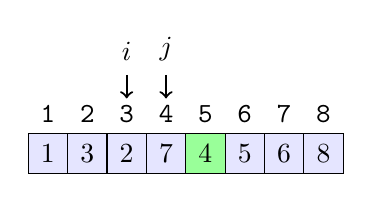
\begin{tikzpicture}
		[	box/.style={rectangle,draw=black, fill=blue!10!white,minimum size=.5cm},
		plain/.style={draw=none,fill=none,font=\ttfamily}
		]
		\node[box] at (.5,0){1};
		\node[box] at (1,0){3};
		\node[box] at (1.5,0){2};
		\node[box] at (2,0){7};
		\node[box,fill=green!40] at (2.5,0){4};
		\node[box] at (3,0){5};
		\node[box] at (3.5,0){6};
		\node[box] at (4,0){8};
\node[plain] at (.5,0.5){1};
\node[plain] at (1,0.5){2};
\node[plain] at (1.5,0.5){3};
\node[plain] at (2,0.5){4};
\node[plain] at (2.5,0.5){5};
\node[plain] at (3,0.5){6};
\node[plain] at (3.5,0.5){7};
\node[plain] at (4,0.5){8};
		\draw[->, thick] (1.5,1) --  node[above,yshift=2mm]{$i$} (1.5,.7);
		\draw[->, thick] (2,1) --  node[above,yshift=2mm]{$j$} (2,.7);
\end{tikzpicture}
\end{center}


Essendo $i<j$ si effettua un'ulteriore ripetizione del blocco e gli indici assumono i valori $i=4,j=3$. La procedura termina restituendo quindi $j=3$. Adesso $q=3$ e tocca invocare le procedure \textsc{QuickSort}$(A,2,3)$ e \textsc{QuickSort}$(A,4,7)$. \textsc{QuickSort}$(A,2,3)$ attiva \textsc{Partiziona}$(A,2,3)$: il pivot è $A[2]=3$ e gli indici iniziali assumono i valori $i=1$ e $j=4$.
	
\begin{center}
	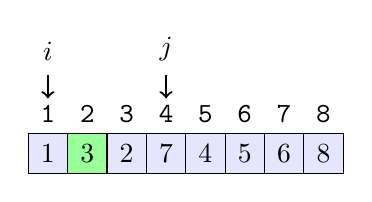
\begin{tikzpicture}
	[	box/.style={rectangle,draw=black, fill=blue!10!white,minimum size=.5cm},
	plain/.style={draw=none,fill=none,font=\ttfamily}
	]
	\node[box] at (.5,0){1};
	\node[box,fill=green!40] at (1,0){3};
	\node[box] at (1.5,0){2};
	\node[box] at (2,0){7};
	\node[box] at (2.5,0){4};
	\node[box] at (3,0){5};
	\node[box] at (3.5,0){6};
	\node[box] at (4,0){8};

\node[plain] at (.5,0.5){1};
\node[plain] at (1,0.5){2};
\node[plain] at (1.5,0.5){3};
\node[plain] at (2,0.5){4};
\node[plain] at (2.5,0.5){5};
\node[plain] at (3,0.5){6};
\node[plain] at (3.5,0.5){7};
\node[plain] at (4,0.5){8};
	\draw[->, thick] (.5,1) --  node[above,yshift=2mm]{$i$} (.5,.7);
	\draw[->, thick] (2,1) --  node[above,yshift=2mm]{$j$} (2,.7);
\end{tikzpicture}
	\end{center}


Alla prima ripetizione gli indici $i,j$ assumono i valori $i=2,j=3$ e si esegue lo swap delle celle $A[2]=3$ e $A[3]=2$.

\begin{center}
		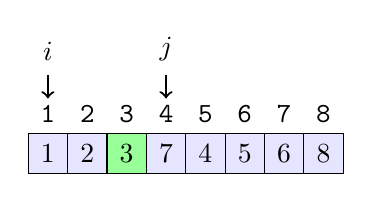
\begin{tikzpicture}
		[	box/.style={rectangle,draw=black, fill=blue!10!white,minimum size=.5cm},
		plain/.style={draw=none,fill=none,font=\ttfamily}
		]
		\node[box] at (.5,0){1};
		\node[box] at (1,0){2};
		\node[box,fill=green!40] at (1.5,0){3};
		\node[box] at (2,0){7};
		\node[box] at (2.5,0){4};
		\node[box] at (3,0){5};
		\node[box] at (3.5,0){6};
		\node[box] at (4,0){8};

\node[plain] at (.5,0.5){1};
\node[plain] at (1,0.5){2};
\node[plain] at (1.5,0.5){3};
\node[plain] at (2,0.5){4};
\node[plain] at (2.5,0.5){5};
\node[plain] at (3,0.5){6};
\node[plain] at (3.5,0.5){7};
\node[plain] at (4,0.5){8};
		\draw[->, thick] (.5,1) --  node[above,yshift=2mm]{$i$} (.5,.7);
		\draw[->, thick] (2,1) --  node[above,yshift=2mm]{$j$} (2,.7);
	\end{tikzpicture}
\end{center}
Alla ripetizione successiva $i=3$ e $j=2$ e la procedura termina restituendo $j=2$. A questo punto si continua con la procedura \textsc{QuickSort}$(A,4,7)$ che invoca \textsc{Partiziona}$(A,4,7)$ il quale imposta il pivot nella cella $A[4]=7$ e gli indici $i,j$ assumono i valori $i=3$ e $j=8$.

\begin{center}
		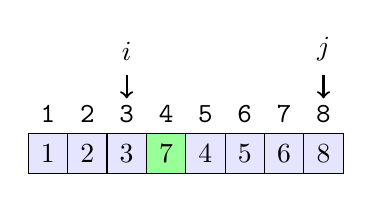
\begin{tikzpicture}
	[	box/.style={rectangle,draw=black, fill=blue!10!white,minimum size=.5cm},
	plain/.style={draw=none,fill=none,font=\ttfamily}
	]
	\node[box] at (.5,0){1};
	\node[box] at (1,0){2};
	\node[box] at (1.5,0){3};
	\node[box,fill=green!40] at (2,0){7};
	\node[box] at (2.5,0){4};
	\node[box] at (3,0){5};
	\node[box] at (3.5,0){6};
	\node[box] at (4,0){8};

\node[plain] at (.5,0.5){1};
\node[plain] at (1,0.5){2};
\node[plain] at (1.5,0.5){3};
\node[plain] at (2,0.5){4};
\node[plain] at (2.5,0.5){5};
\node[plain] at (3,0.5){6};
\node[plain] at (3.5,0.5){7};
\node[plain] at (4,0.5){8};
	\draw[->, thick] (1.5,1) --  node[above,yshift=2mm]{$i$} (1.5,.7);
	\draw[->, thick] (4,1) --  node[above,yshift=2mm]{$j$} (4,.7);
\end{tikzpicture}
	\end{center}

Alla prima ripetizione gli indici assumono i valori $i=4,j=7$ e si effettua lo swap delle celle $A[4]=7$ e $A[7]=6$.
	
\begin{center}
	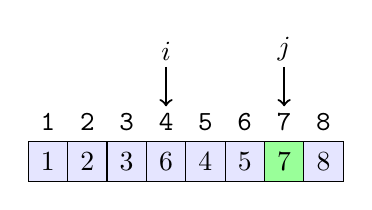
\begin{tikzpicture}
		[	box/.style={rectangle,draw=black, fill=blue!10!white,minimum size=.5cm},
		plain/.style={draw=none,fill=none,font=\ttfamily}
		]
		\node[box] at (.5,0){1};
		\node[box] at (1,0){2};
		\node[box] at (1.5,0){3};
		\node[box] at (2,0){6};
		\node[box] at (2.5,0){4};
		\node[box] at (3,0){5};
		\node[box,fill=green!40] at (3.5,0){7};
		\node[box] at (4,0){8};

\node[plain] at (.5,0.5){1};
\node[plain] at (1,0.5){2};
\node[plain] at (1.5,0.5){3};
\node[plain] at (2,0.5){4};
\node[plain] at (2.5,0.5){5};
\node[plain] at (3,0.5){6};
\node[plain] at (3.5,0.5){7};
\node[plain] at (4,0.5){8};
		\draw[->, thick] (2,1.2) --  node[above,yshift=2mm]{$i$} (2,.7);
		\draw[->, thick] (3.5,1.2) --  node[above,yshift=2mm]{$j$} (3.5,.7);
	\end{tikzpicture}
\end{center}

Nella ripetizione successiva si raggiunge la condizione di uscita con $i=7$ e $j=6$ e la procedura restituisce $j=6$. A questo punto si chiama \textsc{Quicksort}$(A,4,6)$ il quale a sua volta invoca \textsc{Partiziona}$(A,4,6)$. Il pivot selezionato è $A[4]=6$, gli indici inizialmente assumono i valori $i=3$ e $j=7$:
	
\begin{center}
	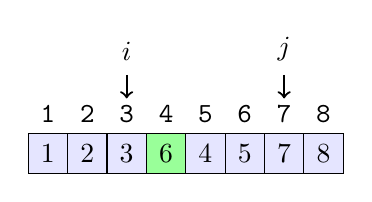
\begin{tikzpicture}
	[	box/.style={rectangle,draw=black, fill=blue!10!white,minimum size=.5cm},
	plain/.style={draw=none,fill=none,font=\ttfamily}
	]
	\node[box] at (.5,0){1};
	\node[box] at (1,0){2};
	\node[box] at (1.5,0){3};
	\node[box,fill=green!40] at (2,0){6};
	\node[box] at (2.5,0){4};
	\node[box] at (3,0){5};
	\node[box] at (3.5,0){7};
	\node[box] at (4,0){8};
\node[plain] at (.5,0.5){1};
\node[plain] at (1,0.5){2};
\node[plain] at (1.5,0.5){3};
\node[plain] at (2,0.5){4};
\node[plain] at (2.5,0.5){5};
\node[plain] at (3,0.5){6};
\node[plain] at (3.5,0.5){7};
\node[plain] at (4,0.5){8};
	\draw[->, thick] (1.5,1) --  node[above,yshift=2mm]{$i$} (1.5,.7);
	\draw[->, thick] (3.5,1) --  node[above,yshift=2mm]{$j$} (3.5,.7);
\end{tikzpicture}
\end{center}

Alla prima ripetizione gli indici assumono i valori $i=4$ e $j=6$ e si swappano le celle $A[4]=6$ e $A[6]=5$:
\begin{center}
	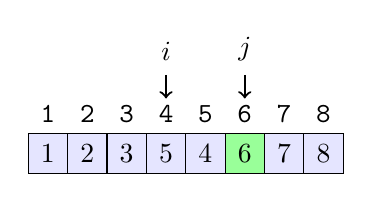
\begin{tikzpicture}
		[	box/.style={rectangle,draw=black, fill=blue!10!white,minimum size=.5cm},
		plain/.style={draw=none,fill=none,font=\ttfamily}
		]
		\node[box] at (.5,0){1};
		\node[box] at (1,0){2};
		\node[box] at (1.5,0){3};
		\node[box] at (2,0){5};
		\node[box] at (2.5,0){4};
		\node[box,fill=green!40] at (3,0){6};
		\node[box] at (3.5,0){7};
		\node[box] at (4,0){8};

\node[plain] at (.5,0.5){1};
\node[plain] at (1,0.5){2};
\node[plain] at (1.5,0.5){3};
\node[plain] at (2,0.5){4};
\node[plain] at (2.5,0.5){5};
\node[plain] at (3,0.5){6};
\node[plain] at (3.5,0.5){7};
\node[plain] at (4,0.5){8};
		\draw[->, thick] (2,1) --  node[above,yshift=2mm]{$i$} (2,.7);
		\draw[->, thick] (3,1) --  node[above,yshift=2mm]{$j$} (3,.7);
	\end{tikzpicture}
\end{center}


Alla seconda ripetizione si raggiunge la condizione di uscita e si restituisce $j=5$. A questo punto \textsc{QuickSort}$(A,4,5)$ invoca \textsc{Partiziona}$(A,4,5)$, il pivot diventa $A[4]=5$ mentre gli indici $i,j$ assumono i valori $i=3$ e $j=6$:
\begin{center}
		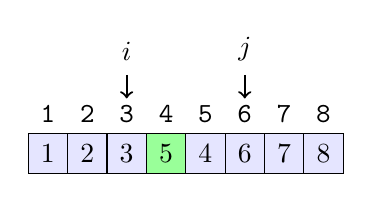
\begin{tikzpicture}
		[	box/.style={rectangle,draw=black, fill=blue!10!white,minimum size=.5cm},
		plain/.style={draw=none,fill=none,font=\ttfamily}
		]
		\node[box] at (.5,0){1};
		\node[box] at (1,0){2};
		\node[box] at (1.5,0){3};
		\node[box,fill=green!40] at (2,0){5};
		\node[box] at (2.5,0){4};
		\node[box] at (3,0){6};
		\node[box] at (3.5,0){7};
		\node[box] at (4,0){8};

\node[plain] at (.5,0.5){1};
\node[plain] at (1,0.5){2};
\node[plain] at (1.5,0.5){3};
\node[plain] at (2,0.5){4};
\node[plain] at (2.5,0.5){5};
\node[plain] at (3,0.5){6};
\node[plain] at (3.5,0.5){7};
\node[plain] at (4,0.5){8};
		\draw[->, thick] (1.5,1) --  node[above,yshift=2mm]{$i$} (1.5,.7);
		\draw[->, thick] (3,1) --  node[above,yshift=2mm]{$j$} (3,.7);
	\end{tikzpicture}

\end{center}

A questo punto, durante la prima ripetizione di \textsc{Partiziona}$(A,4,5)$ gli indici assumono i valori $i=4$ e $j=5$ e si esegue lo scambio di $A[4]=5$ e $A[5]=4$:
\begin{center}
		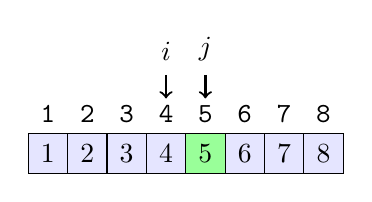
\begin{tikzpicture}
		[	box/.style={rectangle,draw=black, fill=blue!10!white,minimum size=.5cm},
		plain/.style={draw=none,fill=none,font=\ttfamily}
		]
		\node[box] at (.5,0){1};
		\node[box] at (1,0){2};
		\node[box] at (1.5,0){3};
		\node[box] at (2,0){4};
		\node[box,fill=green!40] at (2.5,0){5};
		\node[box] at (3,0){6};
		\node[box] at (3.5,0){7};
		\node[box] at (4,0){8};
\node[plain] at (.5,0.5){1};
\node[plain] at (1,0.5){2};
\node[plain] at (1.5,0.5){3};
\node[plain] at (2,0.5){4};
\node[plain] at (2.5,0.5){5};
\node[plain] at (3,0.5){6};
\node[plain] at (3.5,0.5){7};
\node[plain] at (4,0.5){8};
		\draw[->, thick] (2,1) --  node[above,yshift=2mm]{$i$} (2,.7);
		\draw[->, thick] (2.5,1) --  node[above,yshift=2mm]{$j$} (2.5,.7);
	\end{tikzpicture}
\end{center}

Infine nella ripetizione successiva si raggiunge la condizione di uscita e l'algoritmo termina ottenendo così l'array ordinato:

\begin{center}
	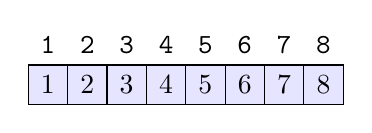
\begin{tikzpicture}
		[	box/.style={rectangle,draw=black, fill=blue!10!white,minimum size=.5cm},
		plain/.style={draw=none,fill=none,font=\ttfamily}
		]
		\node[box] at (.5,0){1};
		\node[box] at (1,0){2};
		\node[box] at (1.5,0){3};
		\node[box] at (2,0){4};
		\node[box] at (2.5,0){5};
		\node[box] at (3,0){6};
		\node[box] at (3.5,0){7};
		\node[box] at (4,0){8};

\node[plain] at (.5,0.5){1};
\node[plain] at (1,0.5){2};
\node[plain] at (1.5,0.5){3};
\node[plain] at (2,0.5){4};
\node[plain] at (2.5,0.5){5};
\node[plain] at (3,0.5){6};
\node[plain] at (3.5,0.5){7};
\node[plain] at (4,0.5){8};
	\end{tikzpicture}

\end{center}

\subsubsection{Correttezza dell'algoritmo \textsc{Partiziona}}
Al ritorno  di \textsc{Partiziona} (Algoritmo \ref{alg:partiziona}) la variabile restituita $j$ deve soddisfare la proprietà \ref{prop:quicksortpartiziona} per garantire la correttezza dell'algoritmo, ovvero:
\begin{displaymath}
	p \leq j <r
\end{displaymath}
Per verificare ciò basta dimostrare che siano impossibili i seguenti casi:
\begin{eqnarray}
	j < p \\ \label{qsimp1}
	j \geq r  \label{qsimp2}
\end{eqnarray}
Per fare ciò basta verificare che non si verificano i casi:
\begin{itemize}
	\item $j=p-1$, essendo $i=p-1$, è l'unico $j<p$ che potrebbe verificarsi vista la scrittura del nostro algoritmo;
	\item $j=r$, anche se $j=r+1$ l'algoritmo \ref{alg:partiziona} fa almeno un decremento sulla variabile $j$.
\end{itemize}

\paragraph{Prima dimostrazione}
Partendo dal secondo punto, dimostriamo che $j$ non può mai assumere il valore $r$. Per restituire $j=r$ significa che gli indici $i$ e $j$ si sono incrociati su $r$.

Notiamo il fatto che $j$ può fermarsi sul valore $r$ solo nella prima iterazione del \texttt{repeat} esterno. Quindi bisogna dimostrare che l'indice $i$ non arrivi mai ad $r$ essendo questo l'unico modo che ha per uscire dal ciclo con $j=r$.

Alla prima iterazione del \texttt{repeat-until} esterno l'indice $j$ viene decrementato ad $r$ ed essendo falsa la condizione $A[r]\leq A[p]=x$ l'algoritmo passa alla linea 8 effettuando un incremento dell'indice $i$ portandolo a $i=p$.

A questo punto si esce dal secondo blocco \texttt{repeat-until} e l'esecuzione passa alla linea 11 che esegue lo scambio tra $A[p]$ e $A[r]$. Dato che $i=p$ e $j=r$ con $p<r$ verrà eseguita una seconda iterazione del \texttt{repeat-until} esterno che decrementerà nuovamente l'indice $j$.
\begin{flushright}
	\blacksquare
\end{flushright}

\paragraph{Seconda dimostrazione}
Per dimostrare che  $j \neq p-1$ basta garantire che il primo \texttt{repeat-until} interno non si ripeta all'infinito.

Poiché non possiamo garantire di essere alla prima iterazione non è detto che $x$ sia ancora nella prima posizione della sequenza poiché potrebbero esserci stati degli scambi, ma se questi sono avvenuti significa certamente che in $A[p]$ c’è un valore minore od uguale a $x$ e ciò garantisce che $j$ si fermerà sicuramente in $p$ (questo è un ragionamento molto astratto, infatti se ci sono stati degli scambi allora $i > p$ e quindi $j$ si fermerà sicuramente prima di arrivare a $p$ essendo la condizione di uscita).

Ora poiché la variabile $i$ può essere solo incrementata è evidente che non potrà essere minore di $p$ ma allora ciò significa che se $j$ arriva a $p$ in quella stessa iterazione la condizione $i \geq j$ sarà verificata e l’algoritmo terminerà con un valore $j \geq p$.
\begin{flushright}
	\blacksquare
\end{flushright}

\subsubsection{Ordinamento}
L'algoritmo \textsc{Partiziona} garantisce che, alla sua terminazione, siano verificate le seguenti proprietà:
\begin{eqnarray}
	\forall \ z: p \leq z \leq j \qquad A[z]\leq x\\
	\forall \ t: j+1 \leq t \leq r \qquad A[t]\geq x
\end{eqnarray}
Queste ultime due possono essere unite in:
\begin{equation}
	\forall \ z,t: p \leq z \leq j < t \leq r \qquad A[z]\leq x \leq A[t]
\end{equation}
che rappresenta la proprietà da garantire:
\begin{equation}
	\forall \ i: p \leq i \leq q \ \wedge \ \forall \ j: \ q+1 \leq j \leq r \qquad A[i]\leq A[j]
\end{equation}

\subsection{Prestazioni di \textsc{QuickSort}}
Le tecniche viste fino a questo momento per studiare il costo computazionale degli algoritmi cercano di calcolare il costo di ogni linea e moltiplicarlo per il numero di esecuzioni. Nel caso del \textsc{QuickSort} il costo dell'algoritmo dipende dalla bontà dell'input. Facendo però delle analisi a priori è possibile trovare un limite asintotico superiore per \textsc{Partiziona}. Infatti, sapendo che $p<r$ si ha che la somma dei \texttt{repeat-until} interni sarà $n + 1$ o $n + 2$ (poiché l’algoritmo praticamente termina o con $i = j$ se l’input è dispari oppure con $i = j + 1$ se l’input è pari) mentre il corpo dell’if al massimo viene eseguito per $n/2$ volte e dunque:
\begin{equation}
	T_{Partiziona}=\Theta(n)+O(n)=\Theta(n)
\end{equation}

Scrivendo l'equazione di ricorrenza di \textsc{QuickSort} si ha:
\begin{equation}\label{eqric:quicksort}
	T_{QuickSort}(n)=
	\left \{
	\begin{array}{lc}
		\Theta(1) & \mbox{se } n \leq 1 \\
		T_{QuickSort}(q)+ T_{QuickSort}(n-q) + T_{Partiziona}(n) & \mbox{se } n >1
	\end{array}
	\right.
\end{equation}

\subsubsection{Caso migliore e caso peggiore per \textsc{QuickSort}}
A causa dell'algoritmo \textsc{Partiziona} non è possibile sapere a priori come viene diviso l’input tra le due chiamate poiché dipende da come
viene scelto il pivot e dall’istanza di input. Ma posso fare i seguenti ragionamenti:
\begin{itemize}
	\item Se tutti gli elementi sono uguali \textsc{Partiziona} divide la sequenza in due parti quasi uguali;
	In questo caso $q= \lfloor n/2 \rfloor$ e si ha $T_{QuickSort}(n)=\Theta(n \log n)$ essendo
	\begin{equation}\label{eqric:istanza1qs}
		T_{QuickSort}(n)=
		\left \{
		\begin{array}{lc}
			\Theta(1) & \mbox{se } n \leq 1 \\
			T_{QuickSort}(\frac{n}{2})+ T_{QuickSort}(\frac{n}{2}) + \Theta(n) & \mbox{se } n >1
		\end{array}
		\right.
	\end{equation}
	come visto per \textsc{MergeSort} in \ref{eqric:mergesort}.
	\item Se invece si ha in input una sequenza già ordinata, questa viene suddivisa in una partizione da un solo elemento (quella di sinistra) e l'altra con gli elementi restanti.
	In questo caso si avrà:
	\begin{equation}\label{eqric:istanza2qs}
		T_{QuickSort}(n)=
		\left \{
		\begin{array}{lc}
			\Theta(1) & \mbox{se } n \leq 1 \\
			T_{QuickSort}(1)+ T_{QuickSort}(n-1) + \Theta(n) & \mbox{se } n >1
		\end{array}
		\right.
	\end{equation}
	e quindi $T_{QuickSort}(n)= \Theta(n^{2})$ come visto nell'esempio del calcolo del fattoriale in \ref{eq:fattoriale}.
\end{itemize}

Da questi brevi calcoli si ottengono funzioni che non coincidono asintoticamente. C'è da chiedersi se queste due tipologie di istanze rappresentano il caso migliore e il caso peggiore per questo algoritmo. Si osserva che qualsiasi istanziazione dell'equazione di ricorrenza \ref{eqric:quicksort} genererà sempre un albero binario completo diverso che avrà sempre un numero fissato di foglie, ovvero tante quanti sono gli elementi da ordinare. Cioè:
\begin{displaymath}
	\begin{array}{lc}
		\#_{foglie}=n \\
		\#_{nodi}=2n-1
	\end{array}
\end{displaymath}

Fino a questo momento abbiamo ottenuto la funzione che risolve la funzione di ricorrenza lavorando sull'albero di ricorsione che ne deriva: sommando, livello per livello, i contributi si otteneva il costo totale. Dato che \textsc{Partiziona} divide la sequenza in due parti di grandezza $q$ ed $n-q$ si avrà che ogni livello avrà sempre un costo lineare e quindi ci aspetteremo di ottenere costi più alti al crescere dell'altezza degli alberi, al variare dell'albero di ricorrenza. Consideriamo il caso dell'albero generato dall'equazione di ricorrenza \ref{eqric:istanza2qs} mostrato in figura \ref{fig:alberoricorrenzaist2qs}.

\begin{center}
	\begin{tikzpicture}
		\node{$n$}
		child{
			node{1}
		}
		child{
			node{$n-1$}
			child{
				node{1}
			}
			child{
				node{$n-2$}
				child{
					node{1}
				}
				child{
					node{$n-3$}
					child{
						node{1}
					}
					child{
						node{$\ddots$}
						child[missing]
						child{
							node{1}
						}
					}
				}
			}
		};
	\end{tikzpicture}
	\captionof{figure}{Albero di ricorrenza dell'equazione \ref{eqric:istanza2qs}}\label{fig:alberoricorrenzaist2qs}
\end{center}

Per questo tipo di albero il livello 0 e il livello 1 hanno lo stesso contributo, però dal livello 2 in poi il contributo di ogni livello è pari a:
\begin{displaymath}
	\forall \ l \geq 1 \qquad Costo_{l}=n-l+1
\end{displaymath}
Di conseguenza il tempo di esecuzione sarà:
\begin{equation}
	T(n)= n + \sum_{l=1}^{n} (n-l+1) = \Theta(n^{2})
\end{equation}

Nel caso dell'equazione \ref{eqric:istanza1qs} l'albero di ricorrenza è fatto come mostrato in figura \ref{fig:alberoricorrenzaist1qs}. E il costo sarà dato dall'equazione:
\begin{equation}
	T(n)=\sum_{l=0}^{h}n=n \sum_{l=0}^{h}1= n \log_{2} n
\end{equation}

\begin{center}
	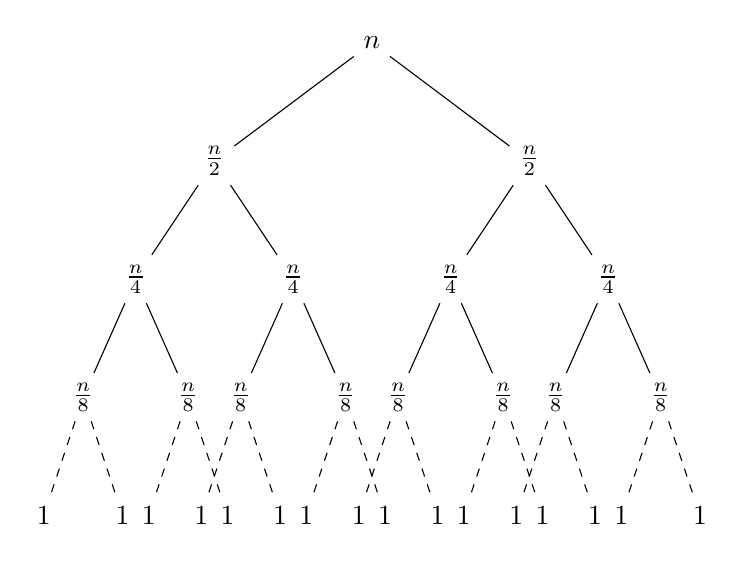
\begin{tikzpicture}
		[level/.style={sibling distance=40mm/#1}]
		\node{$n$}
		child
		{
			node{$\frac{n}{2}$}
			child
			{
				node{$\frac{n}{4}$}
				child
				{
					node{$\frac{n}{8}$}
					child[dashed]
					{
						node{$1$}
					}
					child[dashed]
					{
						node{$1$}
					}
				}
				child
				{
					node{$\frac{n}{8}$}
					child[dashed]
					{
						node{$1$}
					}
					child[dashed]
					{
						node{$1$}
					}
				}
			}
			child
			{
				node{$\frac{n}{4}$}
				child
				{
					node{$\frac{n}{8}$}
					child[dashed]
					{
						node{$1$}
					}
					child[dashed]
					{
						node{$1$}
					}
				}
				child
				{
					node{$\frac{n}{8}$}
					child[dashed]
					{
						node{$1$}
					}
					child[dashed]
					{
						node{$1$}
					}
				}
			}
		}
		child
		{
			node{$\frac{n}{2}$}
			child
			{
				node{$\frac{n}{4}$}
				child
				{
					node{$\frac{n}{8}$}
					child[dashed]
					{
						node{$1$}
					}
					child[dashed]
					{
						node{$1$}
					}
				}
				child
				{
					node{$\frac{n}{8}$}
					child[dashed]
					{
						node{$1$}
					}
					child[dashed]
					{
						node{$1$}
					}
				}
			}
			child
			{
				node{$\frac{n}{4}$}
				child
				{
					node{$\frac{n}{8}$}
					child[dashed]
					{
						node{$1$}
					}
					child[dashed]
					{
						node{$1$}
					}
				}
				child
				{
					node{$\frac{n}{8}$}
					child[dashed]
					{
						node{$1$}
					}
					child[dashed]
					{
						node{$1$}
					}
				}
			}
		};
	\end{tikzpicture}
	\captionof{figure}{Albero di ricorrenza dell'equazione \ref{eqric:istanza1qs}}\label{fig:alberoricorrenzaist1qs}
\end{center}

Si dimostra così che queste due tipologie di alberi rappresentano, nel primo caso, il caso peggiore e il caso migliore per l'algoritmo \textsc{QuickSort}. Essendo le equazioni non coincidenti asintoticamente resta da studiare il caso medio.

\subsubsection{Partizionamento bilanciato}
Il bilanciamento del partizionamento influisce sulla ricorrenza che descrive il tempo di esecuzione.

Supponiamo, per esempio, che l'algoritmo di partizionamento produca sempre una ripartizione proporzionale 3 a 1, che a prima vista potrebbe sembrare molto sbilanciata. In questo caso si ottiene la ricorrenza:
\begin{equation}
	T(n)\leq T(3n/4) + T(n/4) + cn
\end{equation}
sul tempo di esecuzione di \textsc{QuickSort}, dove abbiamo esplicitamente incluso la costante $c$ nascosta nel termine $\Theta(n)$. La Figura \ref{fig:partizionamentobilanciato} illustra l'albero di ricorsione per questa ricorrenza. Notiamo che ogni livello dell'albero ha un costo $cn$, finché non viene raggiunta una condizione al contorno alla profondità $\log_{4} n = \Theta(\lg n)$, dopo la quale i livelli hanno al massimo un costo $cn$.

La ricorsione termina alla profondità $\log_{4/3}n=\Theta(\lg n)$. Il costo totale di \textsc{QuickSort} è dunque $O(n \log n)$. Pertanto, con una ripartizione proporzionale 3 a 1 a ogni livello di ricorsione, che intuitivamente sembra molto vicina al caso peggiore, \textsc{QuickSort} viene eseguito nel tempo $O(n \log n)$ - asintoticamente uguale a quello che si ha nel caso migliore.

In effetti anche una ripartizione 99 a 1 determina un tempo di esecuzione pari a $O(n \log n)$. La ragione è che qualsiasi ripartizione con \textit{proporzionalità costante} produce un albero di ricorsione di profondità $\Theta(\log n)$, dove il costo in ogni livello è lineare.


\begin{center}
 	\begin{tikzpicture}
 		[level/.style={sibling distance=40mm/#1}]
 		\node{$n$}
 		child
 		{
 			node{$n/4$}
 			child
 			{
 				node{$n/16$}
 			}
	 		child
	 		{
	 			node{$3n/16$}
	 		}
 		}
 		child
 		{
 			node{$3n/4$}
 			child
 			{
 				node{$3n/16$}
 			}
 			child
 			{
 				node{$9n/16$}
 				child
 				{
 					node{$9n/16$}
 				}
 				child
 				{
 					node{$27n/16$}
 					child[dashed]
 					{
 						node{$1$}
 					}
 					child[dashed]
 					{
 						node{$1$}
 					}
 				}
 			}
 		};
 	\end{tikzpicture}
	\captionof{figure}{Un'albero di ricorsione per \textsc{QuickSort} quando \textsc{Partiziona} genera sempre una ripartizione 3 a 1, determinando un tempo di esecuzione pari a $O(n \log n)$. I nodi mostrano le dimensioni dei sottoproblemi, con i costi per livello a destra. Questi costi includono la costante $c$ implicita nel termine $\Theta(n)$.}\label{fig:partizionamentobilanciato}
\end{center}

\subsubsection{Analisi del caso medio per \textsc{QuickSort}}
Per trovare una funzione di tempo medio bisogna applicare un'analisi simile a quella vista per il caso medio di \textsc{Insertion-Sort}(Algoritmo \ref{alg:insertsort}). Il nostro obiettivo sarà quello di definire un'equazione di ricorrenza di tempo medio basato su determinate funzioni di tempo medio sui sottoproblemi. Infatti, essendo l'approccio ricorsivo un modo di decomporre il problema, se vogliamo decomporre il tempo medio in istanze di sottoproblemi si deve capire prima quella che deve essere la computazione media locale.

Poiché \textsc{Partiziona} determina un valore $q$ per ogni nodo locale dell'albero di ricorsione, fissato un valore $q$ si determinano ben due sottoproblemi. L'idea sarà quella di generare due sottoproblemi di dimensione $q$ ed $n-q$, fissato un valore $q$. Senza ledere di generalità ragioneremo su delle sequenze che non contengono duplicati\footnote{Maggiori saranno i duplicati uguali al pivot, maggiori saranno le probabilità di avere partizionamenti bilanciati a metà.}. In questo caso, le dimensioni delle partizioni sono univocamente determinate dal \textbf{rango} del pivot.

\dfn{Rango}{Data una sequenza e un pivot $x$, il \textbf{rango} del pivot è il numero di elementi minori o uguali ad $x$ nella sequenza. Di conseguenza, data una sequenza di $n$ valori si ha:
	\begin{displaymath}
		1 \leq r(x) \leq n
	\end{displaymath}
}

\begin{example}
	Sia $A=[1,3,7,9,12,15]$ con $x=1$. Allora il rango di $x$ sarà: $r_{A}(x)=1$
\end{example}

Esiste una corrispondenza tra il rango di x e il valore di q: infatti la scelta del rango determina le dimensioni delle partizioni. Infatti, come si vede nella Tabella \ref{relazionerangopivot}, per $r_{A}(x) \geq 2$ si ha che $q=r_{A}(x)-1$.

\begin{center}
	\begin{tblr}{hlines,vlines,row{1}={primary!80!white}}
		\textbf{$r_{A}(x)$} &q \\
		1 & 1 \\
		2 & 1 \\
		3 & 2 \\
		4 & 3 \\
		$\vdots$ & $\vdots$\\
		$n-1$ & $n-2$ \\
		$n$ & $n$ \\
	\end{tblr}
	\captionof{table}{Corrispondenza tra il rango del pivot e il valore di $q$}\label{relazionerangopivot}
\end{center}

Di fatto scegliere un pivot significa trovare un rango che determina il valore di q. Quindi è possibile pensare di dividere le varie istanze di sequenze di n elementi in tante classi di equivalenza, dove ciascuna classe corrisponde all'insieme delle istanze con un determinato rango.

\begin{center}
	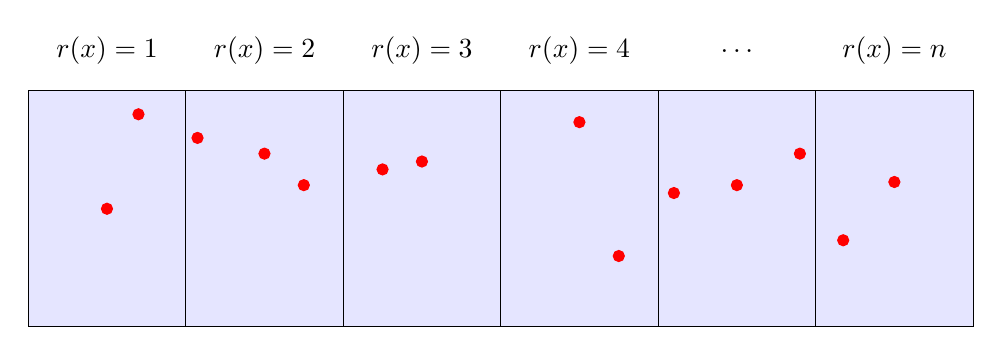
\begin{tikzpicture}
		[	box/.style={rectangle,draw=black, fill=blue!10!white,minimum width=2cm,minimum height=3cm},
		plain/.style={draw=none,fill=none},
		]
		\node[box,name=1] at (1,0){};
		\node[box,name=2] at (3,0){};
		\node[box,name=3] at (5,0){};
		\node[box,name=4] at (7,0){};
		\node[box,name=5] at (9,0){};
		\node[box,name=6] at (11,0){};

		\filldraw[red] (1,0) circle (2pt);
		\filldraw[red] (1.4,1.2) circle (2pt);
		\filldraw[red] (2.15,.9) circle (2pt);
		\filldraw[red] (3,.7) circle (2pt);
		\filldraw[red] (3.5,.3) circle (2pt);
		\filldraw[red] (5,.6) circle (2pt);
		\filldraw[red] (4.5,.5) circle (2pt);
		\filldraw[red] (7,1.1) circle (2pt);
		\filldraw[red] (7.5,-.6) circle (2pt);
		\filldraw[red] (8.2,.2) circle (2pt);
		\filldraw[red] (9,.3) circle (2pt);
		\filldraw[red] (9.8,.7) circle (2pt);
		\filldraw[red] (11,.34) circle (2pt);
		\filldraw[red] (10.35,-.4) circle (2pt);
		\node[plain,yshift=.5cm] at (1.north) {$r(x)=1$};
		\node[plain,yshift=.5cm] at (2.north) {$r(x)=2$};
		\node[plain,yshift=.5cm] at (3.north) {$r(x)=3$};
		\node[plain,yshift=.5cm] at (4.north) {$r(x)=4$};
		\node[plain,yshift=.5cm] at (5.north) {$\ldots$};
		\node[plain,yshift=.5cm] at (6.north) {$r(x)=n$};
	\end{tikzpicture}
	\captionof{figure}{Suddivisioni delle istanze (punti rossi) in classi di equivalenze. Ogni istanza con lo stesso rango appartiene alla stessa classe di equivalenza.}
\end{center}

Fatta questa suddivisione delle istanze posso esprimere il tempo medio come segue:
\begin{equation}\label{equazinetempomedioqs}
	T_{m}(n)=\frac{1}{n}\bigl[ \sum_{r=1}^{n} T_{M}^{r}(n) \bigr]
\end{equation}
dove $T_{M}^{r}(n)$, fissato un rango $r_{A}(x)$, esprime il tempo medio su sequenze di dimensione n.

Ovvero:
\begin{equation}
	T_{M}^{r}(n) = T_{M}(q_{r})+T_{M}(n-q_{r})+ \Theta(n)
\end{equation}

Sostituendo nell'equazione \ref{equazinetempomedioqs} si ottiene:
\begin{equation}\label{eqmediaqs2}
	T_{M}(n) = \frac{\sum_{r=1}^{n} \bigl( T_{M}(q_{r})+ T_{M}(n-q_{r})+\Theta(n) \bigr)}{n}
\end{equation}

È possibile semplificare l'equazione \ref{eqmediaqs2} togliendo la dipendenza dal rango:
\begin{eqnarray}
	T_{M}(n) &=& \frac{1}{n} \Bigl(T_{M}(1)+T_{M}(n-1)+\Theta(n)+ \sum_{r=2}^{n}\bigl(T_{M}(q_{r})+T_{M}(n-q_{r})+\Theta(n)\bigr)\Bigr) \nonumber \\
	&=& \frac{1}{n}\Bigl(\Theta(1)+O(n^{2})+\Theta(n)+\sum_{q=1}^{n-1}\bigl(T_{M}(q)+T_{M}(n-q)+\Theta(n)\bigr)\Bigr) \nonumber \\
	&=& \frac{1}{n}\Bigl(O(n^{2})+ \sum_{q=1}^{n-1}\Theta(n) + 2\cdot \sum_{q=1}^{n-1}T_{M}(q) \Bigr) \nonumber \\
	&=& \frac{1}{n}\Bigl( O(n^{2})+\Theta(n^{2})+2\cdot \sum_{q=1}^{n-1}T_{M}(q)\Bigr) \nonumber \\
	&=& \frac{1}{n}\Bigl(\Theta(n^{2})+2\cdot \sum_{q=1}^{n-1}T_{M}(q)\Bigr) \nonumber \\
	&=& \frac{\Theta(n^{2})}{n}+ \frac{2}{n} \sum_{q=1}^{n-1}T_{M}(q) \nonumber \\
	&=& \Theta(n) + \frac{2}{n} \sum_{q=1}^{n-1}T_{M}(q)
\end{eqnarray}

Resta da trovare una soluzione per l'equazione $T_{M}(q)$. Per farlo useremo il \textbf{metodo di sostituzione}. L'ipotesi alla base del metodo di sostituzione è la seguente:
\begin{equation}
	\exists \ c \Bigl( \forall n \geq 2 (T_{M}(n) \leq cn\log_{2}n)\Bigr)
\end{equation}

\paragraph{Dimostrazione:}
	Si dimostra per induzione:
	\begin{itemize}
		\item \textbf{Caso base:} Sia $n=2$. $T_{M}(2)$ deve essere minore o uguale di una qualche costante c moltiplicato per $\log_{2}2$, ovvero:
		\begin{displaymath}
			T_{M}(2) \leq c \cdot 2 \log_{2} 2 = 2c
		\end{displaymath}
		ma $$T_{M}(2) = \Theta(2) + \frac{2}{2}\sum_{q=1}^{1}T_{M}(q) =\Theta(2)+\Theta(1)$$
		queste due $	\Theta$ sono costanti che discendono da due operazioni diverse dell'algoritmo (una è la costante di \textsc{Partiziona} mentre la seconda è la costante data dal confronto per vedere se siamo in un caso base o meno). Possiamo quindi rinominarle in $k_{1}$ e $k_{2}$:
		\begin{displaymath}
			T_{M}(2)=k_{1}+k_{2}
		\end{displaymath}
		bisogna dimostrare quindi che è vera la proprietà: $$k_{1}+k_{2}=2c$$
		Presa
		\begin{equation}
			c > \frac{k_{1}+k_{2}}{2}
		\end{equation}
		il caso base è soddisfatto.
		\item \textbf{Passo induttivo ($n \geq 2$): }Sia vera la tesi per qualsiasi numero minore di n.
		Si ha \begin{displaymath}
			T_{M}(n)=\Theta(n)+\frac{2}{n}\sum_{q=1}^{n-1}T_{M}(q)
		\end{displaymath}
		Essendo $1 \leq q \leq n-1$ è sicuramente $q <n$ e quindi possiamo maggiorare usando il passo induttivo: $$T_{M}(q) \leq cq \log_{2}q$$  Si ha così:
		\begin{eqnarray}
			T_{M}(n)&=&\Theta(n)+\frac{2}{n}\sum_{q=1}^{n-1}T_{M}(q) \nonumber \\
			&\leq &\Theta(n)+\frac{2}{n}\sum_{q=1}^{n-1}(cq\log_{2}q)
		\end{eqnarray}
		Usando la proprietà \ref{approssimazionesommatorie} si ha poi:
		\begin{eqnarray}
			\Theta(n)+\frac{2}{n}\sum_{q=1}^{n-1}(cq\log_{2}q) &\leq & \Theta(n)+\frac{2c}{n}\bigl(\frac{n^{2}\log n}{2}-\frac{n^{2}}{8}\bigr) \nonumber \\
			&=& \Theta(n)+cn\log n - \frac{cn}{4} \nonumber \\
			&\leq & cn\log n
		\end{eqnarray}
	\end{itemize}

\begin{flushright}
	\blacksquare
\end{flushright}


\begin{propbox}
		Vale la seguente proprietà:
	\begin{equation}\label{approssimazionesommatorie}
		\sum_{q=1}^{n-1} q \log q \leq \frac{n^{2} \log n n}{2} - \frac{n^{2}}{8}
	\end{equation}
\end{propbox}


\begin{proof}
		Si ha:
	\begin{eqnarray*}
		\forall \ i \leq q \leq n-1 \qquad q<n &\Rightarrow  & \log_{2} q \leq \log_{2} n \\
		&\Rightarrow & q \log_{2} q \leq q \log_{2} n \\
		& \Rightarrow & \sum_{q=1}^{n-1} q\log_{2} q \leq \sum_{q=1}^{n-1} q \log_{2} n = \\
		&=& \log_{2} n \sum_{q=1}^{n-1} q \\
		&=& \log_{2} n \bigl( \frac{n(n-1)}{2}\bigr) \\
		&=& \log_{2} n \bigl( \frac{n^{2}-2}{2}\bigr)\\
		&=& \frac{n^{2}\log_{2}n}{2}- \frac{n\log_{2} n}{2}
	\end{eqnarray*}
\end{proof}

Si dimostra in questo modo che l'equazione di ricorrenza \ref{equazinetempomedioqs} ha una soluzione del tipo polilogaritmica:
\begin{equation}
	T_{QS_{m}}=\Theta(n^{2}\log_{2}n)
\end{equation}

\section{Analisi degli algoritmi di ordinamento}
Si dimostra che il \textbf{problema generale dell'ordinamento} non può essere risolto in tempo minore di $\Omega(n \log n)$ se risolto mediante algoritmi \textbf{basati sui confronti}.

Ogni algoritmo di ordinamento per confronti si può vedere come un processo decisionale per individuare una \textit{permutazione ordinata} di una sequenza. Ovvero, dati due elementi $a_{i}$ e $a_{j}$, eseguiamo uno dei test $a_{i}<a_{j}$, $ a_{i}\leq a_{j}$, $a_{i}=a_{j}$, $a_{i}>a_{j}$ oppure $a_{i}>a_{j}$ per determinare il loro ordine relativo. In questa sezione supponiamo, senza perdere di generalità, che tutti gli elementi di input siano distinti. Fatta questa ipotesi, confronti della forma $a_{i}=a_{j}$ sono inutili, quindi possiamo supporre che non saranno fatti confronti di questo tipo.

\subsection{Alberi di decisione}
Gli ordinamenti per confronti possono essere visti astrattamente in termini di \textbf{alberi di decisione}. Un albero di decisione è un albero binario che rappresenta i confronti fra elementi che vengono effettuati da un particolare algoritmo di ordinamento che opera su input di una data dimensione. Il controllo, lo spostamento dei dati e tutti gli altri aspetti dell'algoritmo vengono ignorati.  La figura \ref{fig:alberodecisione} illustra un esempio di albero di decisione che corrisponde all'algoritmo \textsc{Insertion-Sort} che opera su una sequenza di input di tre elementi.

\begin{center}
	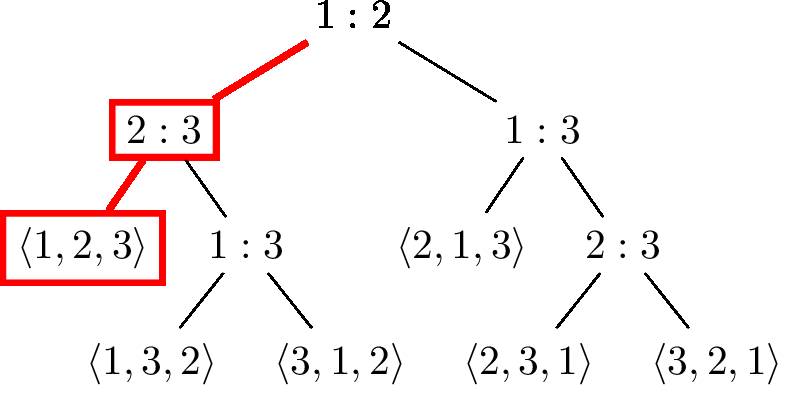
\includegraphics[scale=.35]{res/test.jpg}
	\captionof{figure}{Albero di decisione di un algoritmo che opera su tre elementi.}\label{fig:alberodecisione}
\end{center}

In un albero di decisione, ogni nodo interno è annotato con $i:j$ per qualche $i$ e $j$ nell'intervallo $1 \leq i,j \leq n$, dove $n$ è il numero di elementi nella sequenza di input. Ogni foglia è annotata con una permutazione $\langle \pi(1),\pi(2),...,\pi(n) \rangle$.

L'esecuzione dell'algoritmo di ordinamento corrisponde a tracciare un cammino semplice dalla radice dell'albero di decisione fino a una foglia. Ogni nodo interno rappresenta un confronto $a_{i} \leq a_{j}$. Il sottoalbero sinistro detta i successivi confronti per $a_{i}\leq a_{j}$; il sottoalbero destro detta i successivi confronti per $a_{i}\geq a_{j}$.

Quando raggiunge una foglia, l'algoritmo ha stabilito l'ordinamento $$a_{\pi(1)} \leq a_{\pi(2)} \leq \cdots \leq a_{\pi(n)}$$ Poiché qualsiasi algoritmo di ordinamento corretto deve essere in grado di produrre ogni permutazione del suo input, una \textit{condizione necessaria} affinché un ordinamento per confronti sia corretto è che ciascuna delle $n!$ permutazioni di $n$ elementi appaia come una delle foglie dell'albero di decisione e che ciascuna di queste foglie sia raggiungibile dalla radice attraverso un percorso che corrisponde a una effettiva esecuzione dell'ordinamento per confronti (queste foglie saranno chiamate ``raggiungibili'').

La \textbf{lunghezza del cammino semplice più lungo} dalla radice di un albero di decisione a una delle due foglie raggiungibili rappresenta il \textbf{numero di confronti} che svolge il corrispondente algoritmo di ordinamento nel caso peggiore. Di conseguenza il numero di confronti nel caso peggiore per un dato algoritmo di ordinamento basato sui confronti è \textit{uguale all'altezza del suo albero di decisione.}


\begin{teorbox}
Sia $T$ un albero di decisione che ordina $n$ elementi distinti. $T$ ha un altezza almeno pari a $\Theta(n \log_{2}n)$.
\end{teorbox}


\begin{proof}
	Per quanto detto in precedenza T ha $n!$ foglie, se ne avesse di più sarebbe ridondante, se ne avesse di meno non ha ancora fatto tutti i confronti e quindi sarebbe incompleto. Essendo gli esiti dei confronti solo di due tipi (minore o maggiore) si ha che $T$ è un albero binario (il quale avrà al massimo $2^{h}$ foglie). Da queste informazione possiamo dire dunque che :
	\begin{displaymath}
		n! \leq 2^{h}
	\end{displaymath}
	Per calcolare il tempo medio di un algoritmo basterà quindi dividere la \textbf{lunghezza del percorso esterno} (LPE), ovvero la somma delle lunghezze dei cammini dalla radice alle foglie, per il numero medio di confronti:
	\begin{displaymath}
		T_{M}(n)=\frac{LPE}{n!}
	\end{displaymath}
	Dato un albero saprò calcolare il percorso medio, ma in generale devo trovare un albero che minimizza l'espressione precedente. Poiché non è possibile minimizzare il numero $n$ si può pensare di minimizzare la lunghezza del percorso esterno. Gli alberi completi (vedi \ref{alberi_binari_prop}) rispondono a questa necessità. Infatti questi alberi, fissato un numero di nodi, avranno la minor altezza possibile, minimizzando così la quantità $LPE$.


	In un albero completo valgono le seguenti proprietà:
	\begin{eqnarray}
		N_{h} + N_{h-1} = n!\\
		N_{h} + 2N_{h-1} = 2^{h}
	\end{eqnarray}
	dove $N_{h}$ è il numero di foglie alla profondità $h$ e $N_{h-1}$ è il numero di foglie alla profondità $h$.

	Sottraendo la prima equazione alla seconda si ottiene:
	\begin{equation}
		N_{h-1}= n! - 2^{h}
	\end{equation}
	Abbiamo quindi:
	\begin{eqnarray}
		LPE &=& h \cdot N_{h} + (h-1)N_{h-1} \nonumber \\
		&=& h \cdot N_{h}+ h\cdot N_{h-1} - N_{h-1} \nonumber \\
		&=& h \cdot ( N_{h} + N_{h-1}) - N_{h+1} \nonumber \\
		&=& h \cdot n! - N_{h-1} \nonumber \\
		&=& h \cdot n! - 2^{h} + n!
	\end{eqnarray}

	Il numero medio di confronti sarà allora:
	\begin{eqnarray}
		T_{M}(n)&=&\frac{LPE}{n!} \nonumber \\
		&=& \frac{h \cdot n! - 2^{h} + n!}{n!} \nonumber \\
		&=& h - \frac{2^{h}}{n!}+1 \nonumber
	\end{eqnarray}
	Sapendo che $h= \log n!$ si ha:
	\begin{equation}
		T_{M}(n) = \log n! - \frac{2^{\log n!}}{n!}+1= \log n!
	\end{equation}
	Ma abbiamo già dimostrato che $\log n! = \Theta(n \log n)$ e quindi possiamo concludere dicendo che il tempo di esecuzione di un algoritmo di ordinamento per una sequenza arbitraria di input $n$ non può essere, nel caso medio e nel caso peggiore, migliore di $\Theta(n \log n)$.
\end{proof}


\begin{center}
	\begin{tblr}{hlines,vlines,colspec={lX},row{1}={primary!80!white}}
		\textbf{Algoritmo} & \textbf{Tempo di esecuzione nel caso peggiore} & \textbf{Tempo di esecuzione nel caso medio} \\
		\textbf{\textsc{Insertion Sort}} & $\Theta(n^{2})$ & $\Theta(n^{2})$\\

		\textbf{\textsc{Mergesort}} & $\Theta(n \log n)$& $\Theta(n \log n)$\\

		\textbf{\textsc{Heapsort}} &$O(n \log n)$ & - \\

		\textbf{\textsc{Quicksort}} & $\Theta(n^{2})$ & $\Theta(n \log n)$\\
	\end{tblr}
	\captionof{table}{Confronto dei tempi di esecuzione degli algoritmi di ordinamento}
\end{center}
